% Supplementary material: a separate document, as the journal requires. build.ps1 copies its labels into
% generated/supplement_refs.tex, which main.tex reads.
\documentclass[11pt]{article}
\usepackage[a4paper,margin=2.4cm]{geometry}
\usepackage[T1]{fontenc}
\usepackage[utf8]{inputenc}
\usepackage{lmodern}
\usepackage{microtype}
\usepackage{amsmath,amssymb}
\usepackage{booktabs}
\usepackage{makecell}
\usepackage{adjustbox}
\usepackage{graphicx}
\usepackage{xcolor}
\usepackage[numbers,sort&compress]{natbib}
\usepackage{setspace}
\usepackage[hidelinks]{hyperref}
\usepackage{caption}
\captionsetup{font=small,labelfont=bf}
\newcommand{\authorinput}[1]{\textcolor{red}{\textbf{[#1]}}}

% Every number quoted from the data comes from generated/values.tex (see README.md).
% Generated by careport.psg_assist_manuscript from the committed reports; do not edit.
\expandafter\def\csname val@a1-human-kappa-hi\endcsname{+0.002}
\expandafter\def\csname val@a1-human-kappa-lo\endcsname{\ensuremath{-}0.024}
\expandafter\def\csname val@a1-human-kappa-mean\endcsname{\ensuremath{-}0.010}
\expandafter\def\csname val@a1-human-pct-hi\endcsname{+0.001}
\expandafter\def\csname val@a1-human-pct-lo\endcsname{\ensuremath{-}0.015}
\expandafter\def\csname val@a1-human-pct-mean\endcsname{\ensuremath{-}0.007}
\expandafter\def\csname val@a1-human-share-left\endcsname{61\%}
\expandafter\def\csname val@a1-yasa-kappa-mean\endcsname{\ensuremath{-}0.027}
\expandafter\def\csname val@a1-yasa-kappa-neg\endcsname{4}
\expandafter\def\csname val@a1-yasa-pct-mean\endcsname{\ensuremath{-}0.017}
\expandafter\def\csname val@a1-yasa-pct-neg\endcsname{4}
\expandafter\def\csname val@a1-yasa-share-left\endcsname{67\%}
\expandafter\def\csname val@a1-yasa-sn1-kappa\endcsname{+0.010}
\expandafter\def\csname val@a1-yasa-sn1-pct\endcsname{+0.007}
\expandafter\def\csname val@a1-yasa-sn2-kappa\endcsname{\ensuremath{-}0.027}
\expandafter\def\csname val@a1-yasa-sn2-pct\endcsname{\ensuremath{-}0.021}
\expandafter\def\csname val@a1-yasa-sn3-kappa\endcsname{\ensuremath{-}0.021}
\expandafter\def\csname val@a1-yasa-sn3-pct\endcsname{\ensuremath{-}0.016}
\expandafter\def\csname val@a1-yasa-sn4-kappa\endcsname{\ensuremath{-}0.041}
\expandafter\def\csname val@a1-yasa-sn4-pct\endcsname{\ensuremath{-}0.031}
\expandafter\def\csname val@a1-yasa-sn5-kappa\endcsname{\ensuremath{-}0.055}
\expandafter\def\csname val@a1-yasa-sn5-pct\endcsname{\ensuremath{-}0.024}
\expandafter\def\csname val@a2-arousals-assisted\endcsname{0.788}
\expandafter\def\csname val@a2-arousals-assisted-pct\endcsname{79\%}
\expandafter\def\csname val@a2-arousals-diff\endcsname{+0.575}
\expandafter\def\csname val@a2-arousals-manual\endcsname{0.212}
\expandafter\def\csname val@a2-arousals-n\endcsname{23{,}176}
\expandafter\def\csname val@a2-arousals-rec-max\endcsname{0.76}
\expandafter\def\csname val@a2-arousals-rec-min\endcsname{0.16}
\expandafter\def\csname val@a2-limb-assisted\endcsname{0.988}
\expandafter\def\csname val@a2-limb-assisted-pct\endcsname{99\%}
\expandafter\def\csname val@a2-limb-diff\endcsname{+0.976}
\expandafter\def\csname val@a2-limb-manual\endcsname{0.012}
\expandafter\def\csname val@a2-limb-n\endcsname{11{,}550}
\expandafter\def\csname val@a2-limb-rec-max\endcsname{0.99}
\expandafter\def\csname val@a2-limb-rec-min\endcsname{0.96}
\expandafter\def\csname val@a2-max-pct\endcsname{99\%}
\expandafter\def\csname val@a2-min-pct\endcsname{79\%}
\expandafter\def\csname val@a2-resp-assisted\endcsname{0.951}
\expandafter\def\csname val@a2-resp-assisted-pct\endcsname{95\%}
\expandafter\def\csname val@a2-resp-diff\endcsname{+0.902}
\expandafter\def\csname val@a2-resp-manual\endcsname{0.049}
\expandafter\def\csname val@a2-resp-n\endcsname{27{,}754}
\expandafter\def\csname val@a2-resp-rec-max\endcsname{0.99}
\expandafter\def\csname val@a2-resp-rec-min\endcsname{0.50}
\expandafter\def\csname val@a2-sign-n\endcsname{20}
\expandafter\def\csname val@a2-sign-p\endcsname{\ensuremath{1.9\times10^{-6}}}
\expandafter\def\csname val@a2-sign-pos\endcsname{20}
\expandafter\def\csname val@a2-stages-assisted\endcsname{0.930}
\expandafter\def\csname val@a2-stages-assisted-pct\endcsname{93\%}
\expandafter\def\csname val@a2-stages-diff\endcsname{+0.871}
\expandafter\def\csname val@a2-stages-manual\endcsname{0.058}
\expandafter\def\csname val@a2-stages-n\endcsname{171}
\expandafter\def\csname val@a2-stages-rec-max\endcsname{1.00}
\expandafter\def\csname val@a2-stages-rec-min\endcsname{0.73}
\expandafter\def\csname val@a2-stages-share\endcsname{3.6\%}
\expandafter\def\csname val@a3-arousals-closer\endcsname{1}
\expandafter\def\csname val@a3-limb-closer\endcsname{0}
\expandafter\def\csname val@a3-resp-closer\endcsname{2}
\expandafter\def\csname val@a3-stage-manual\endcsname{0.964}
\expandafter\def\csname val@a3-stage-prefill\endcsname{0.947}
\expandafter\def\csname val@a3-stages-closer\endcsname{3}
\expandafter\def\csname val@a3-units-n\endcsname{20}
\expandafter\def\csname val@a3-units-p\endcsname{0.12}
\expandafter\def\csname val@a3-units-pos\endcsname{6}
\expandafter\def\csname val@b1-gap-d0\endcsname{0.108}
\expandafter\def\csname val@b1-gap-d0-bias\endcsname{+0.059}
\expandafter\def\csname val@b1-gap-d0s\endcsname{0.112}
\expandafter\def\csname val@b1-gap-d0s-bias\endcsname{+0.063}
\expandafter\def\csname val@b1-gap-f1-d1\endcsname{0.117}
\expandafter\def\csname val@b1-gap-f1-d2\endcsname{0.089}
\expandafter\def\csname val@b1-gap-f1-n\endcsname{49}
\expandafter\def\csname val@b1-gap-f10-d1\endcsname{0.035}
\expandafter\def\csname val@b1-gap-f10-d2\endcsname{0.027}
\expandafter\def\csname val@b1-gap-f10-n\endcsname{486}
\expandafter\def\csname val@b1-gap-f2-d1\endcsname{0.082}
\expandafter\def\csname val@b1-gap-f2-d2\endcsname{0.062}
\expandafter\def\csname val@b1-gap-f2-n\endcsname{97}
\expandafter\def\csname val@b1-gap-f20-d1\endcsname{0.024}
\expandafter\def\csname val@b1-gap-f20-d2\endcsname{0.018}
\expandafter\def\csname val@b1-gap-f20-n\endcsname{972}
\expandafter\def\csname val@b1-gap-f5-d1\endcsname{0.051}
\expandafter\def\csname val@b1-gap-f5-d2\endcsname{0.039}
\expandafter\def\csname val@b1-gap-f5-n\endcsname{243}
\expandafter\def\csname val@b1-gap-narrower\endcsname{24\%}
\expandafter\def\csname val@b1-gap-target\endcsname{0.049}
\expandafter\def\csname val@b1-pop\endcsname{4{,}857}
\expandafter\def\csname val@b1-prefill-d0\endcsname{0.947}
\expandafter\def\csname val@b1-prefill-d0-bias\endcsname{+0.048}
\expandafter\def\csname val@b1-prefill-d0s\endcsname{0.975}
\expandafter\def\csname val@b1-prefill-d0s-bias\endcsname{+0.077}
\expandafter\def\csname val@b1-prefill-f1-d1\endcsname{0.084}
\expandafter\def\csname val@b1-prefill-f1-d2\endcsname{0.056}
\expandafter\def\csname val@b1-prefill-f1-n\endcsname{49}
\expandafter\def\csname val@b1-prefill-f10-d1\endcsname{0.025}
\expandafter\def\csname val@b1-prefill-f10-d2\endcsname{0.017}
\expandafter\def\csname val@b1-prefill-f10-n\endcsname{486}
\expandafter\def\csname val@b1-prefill-f2-d1\endcsname{0.059}
\expandafter\def\csname val@b1-prefill-f2-d2\endcsname{0.039}
\expandafter\def\csname val@b1-prefill-f2-n\endcsname{97}
\expandafter\def\csname val@b1-prefill-f20-d1\endcsname{0.017}
\expandafter\def\csname val@b1-prefill-f20-d2\endcsname{0.011}
\expandafter\def\csname val@b1-prefill-f20-n\endcsname{972}
\expandafter\def\csname val@b1-prefill-f5-d1\endcsname{0.037}
\expandafter\def\csname val@b1-prefill-f5-d2\endcsname{0.025}
\expandafter\def\csname val@b1-prefill-f5-n\endcsname{243}
\expandafter\def\csname val@b1-prefill-narrower\endcsname{33\%}
\expandafter\def\csname val@b1-prefill-target\endcsname{0.898}
\expandafter\def\csname val@b1-smallest-f\endcsname{5\%}
\expandafter\def\csname val@b1-yasa-d0\endcsname{0.839}
\expandafter\def\csname val@b1-yasa-d0-bias\endcsname{\ensuremath{-}0.011}
\expandafter\def\csname val@b1-yasa-d0s\endcsname{0.864}
\expandafter\def\csname val@b1-yasa-d0s-bias\endcsname{+0.014}
\expandafter\def\csname val@b1-yasa-f1-d1\endcsname{0.099}
\expandafter\def\csname val@b1-yasa-f1-d2\endcsname{0.061}
\expandafter\def\csname val@b1-yasa-f1-n\endcsname{49}
\expandafter\def\csname val@b1-yasa-f10-d1\endcsname{0.030}
\expandafter\def\csname val@b1-yasa-f10-d2\endcsname{0.018}
\expandafter\def\csname val@b1-yasa-f10-n\endcsname{486}
\expandafter\def\csname val@b1-yasa-f2-d1\endcsname{0.070}
\expandafter\def\csname val@b1-yasa-f2-d2\endcsname{0.043}
\expandafter\def\csname val@b1-yasa-f2-n\endcsname{97}
\expandafter\def\csname val@b1-yasa-f20-d1\endcsname{0.020}
\expandafter\def\csname val@b1-yasa-f20-d2\endcsname{0.012}
\expandafter\def\csname val@b1-yasa-f20-n\endcsname{972}
\expandafter\def\csname val@b1-yasa-f5-d1\endcsname{0.044}
\expandafter\def\csname val@b1-yasa-f5-d2\endcsname{0.027}
\expandafter\def\csname val@b1-yasa-f5-n\endcsname{243}
\expandafter\def\csname val@b1-yasa-narrower\endcsname{39\%}
\expandafter\def\csname val@b1-yasa-target\endcsname{0.850}
\expandafter\def\csname val@b2-a0-n50k-d0\endcsname{0.000}
\expandafter\def\csname val@b2-a0-n50k-d0s\endcsname{0.000}
\expandafter\def\csname val@b2-a0-n50k-d1-01\endcsname{0.500}
\expandafter\def\csname val@b2-a0-n50k-d1-02\endcsname{0.500}
\expandafter\def\csname val@b2-a0-n50k-d1-05\endcsname{0.500}
\expandafter\def\csname val@b2-a0-n50k-d1-1\endcsname{0.500}
\expandafter\def\csname val@b2-a0-n50k-d1-2\endcsname{0.500}
\expandafter\def\csname val@b2-a0-n50k-d2-01\endcsname{0.500}
\expandafter\def\csname val@b2-a0-n50k-d2-02\endcsname{0.500}
\expandafter\def\csname val@b2-a0-n50k-d2-05\endcsname{0.500}
\expandafter\def\csname val@b2-a0-n50k-d2-1\endcsname{0.500}
\expandafter\def\csname val@b2-a0-n50k-d2-2\endcsname{0.500}
\expandafter\def\csname val@b2-a0-n50k-gap-d0\endcsname{\ensuremath{-}0.071}
\expandafter\def\csname val@b2-a0-n50k-gap-d0s\endcsname{\ensuremath{-}0.068}
\expandafter\def\csname val@b2-a0-n50k-gap-unassisted\endcsname{0.000}
\expandafter\def\csname val@b2-a0-n5k-d0\endcsname{0.000}
\expandafter\def\csname val@b2-a0-n5k-d0s\endcsname{0.000}
\expandafter\def\csname val@b2-a0-n5k-d1-01\endcsname{0.500}
\expandafter\def\csname val@b2-a0-n5k-d1-02\endcsname{0.500}
\expandafter\def\csname val@b2-a0-n5k-d1-05\endcsname{0.500}
\expandafter\def\csname val@b2-a0-n5k-d1-1\endcsname{0.500}
\expandafter\def\csname val@b2-a0-n5k-d1-2\endcsname{0.500}
\expandafter\def\csname val@b2-a0-n5k-d2-01\endcsname{0.500}
\expandafter\def\csname val@b2-a0-n5k-d2-02\endcsname{0.500}
\expandafter\def\csname val@b2-a0-n5k-d2-05\endcsname{0.500}
\expandafter\def\csname val@b2-a0-n5k-d2-1\endcsname{0.500}
\expandafter\def\csname val@b2-a0-n5k-d2-2\endcsname{0.500}
\expandafter\def\csname val@b2-a0-n5k-gap-d0\endcsname{\ensuremath{-}0.071}
\expandafter\def\csname val@b2-a0-n5k-gap-d0s\endcsname{\ensuremath{-}0.068}
\expandafter\def\csname val@b2-a0-n5k-gap-unassisted\endcsname{0.000}
\expandafter\def\csname val@b2-a1-n50k-d0\endcsname{0.000}
\expandafter\def\csname val@b2-a1-n50k-d0s\endcsname{0.000}
\expandafter\def\csname val@b2-a1-n50k-d1-01\endcsname{0.668}
\expandafter\def\csname val@b2-a1-n50k-d1-02\endcsname{0.730}
\expandafter\def\csname val@b2-a1-n50k-d1-05\endcsname{0.834}
\expandafter\def\csname val@b2-a1-n50k-d1-1\endcsname{0.915}
\expandafter\def\csname val@b2-a1-n50k-d1-2\endcsname{0.974}
\expandafter\def\csname val@b2-a1-n50k-d2-01\endcsname{0.672}
\expandafter\def\csname val@b2-a1-n50k-d2-02\endcsname{0.736}
\expandafter\def\csname val@b2-a1-n50k-d2-05\endcsname{0.840}
\expandafter\def\csname val@b2-a1-n50k-d2-1\endcsname{0.920}
\expandafter\def\csname val@b2-a1-n50k-d2-2\endcsname{0.976}
\expandafter\def\csname val@b2-a1-n50k-gap-d0\endcsname{\ensuremath{-}0.064}
\expandafter\def\csname val@b2-a1-n50k-gap-d0s\endcsname{\ensuremath{-}0.062}
\expandafter\def\csname val@b2-a1-n50k-gap-unassisted\endcsname{+0.008}
\expandafter\def\csname val@b2-a1-n5k-d0\endcsname{0.000}
\expandafter\def\csname val@b2-a1-n5k-d0s\endcsname{0.000}
\expandafter\def\csname val@b2-a1-n5k-d1-01\endcsname{0.554}
\expandafter\def\csname val@b2-a1-n5k-d1-02\endcsname{0.577}
\expandafter\def\csname val@b2-a1-n5k-d1-05\endcsname{0.620}
\expandafter\def\csname val@b2-a1-n5k-d1-1\endcsname{0.668}
\expandafter\def\csname val@b2-a1-n5k-d1-2\endcsname{0.730}
\expandafter\def\csname val@b2-a1-n5k-d2-01\endcsname{0.556}
\expandafter\def\csname val@b2-a1-n5k-d2-02\endcsname{0.579}
\expandafter\def\csname val@b2-a1-n5k-d2-05\endcsname{0.624}
\expandafter\def\csname val@b2-a1-n5k-d2-1\endcsname{0.672}
\expandafter\def\csname val@b2-a1-n5k-d2-2\endcsname{0.735}
\expandafter\def\csname val@b2-a1-n5k-gap-d0\endcsname{\ensuremath{-}0.064}
\expandafter\def\csname val@b2-a1-n5k-gap-d0s\endcsname{\ensuremath{-}0.062}
\expandafter\def\csname val@b2-a1-n5k-gap-unassisted\endcsname{+0.008}
\expandafter\def\csname val@b2-a2-n50k-d0\endcsname{0.000}
\expandafter\def\csname val@b2-a2-n50k-d0s\endcsname{0.000}
\expandafter\def\csname val@b2-a2-n50k-d1-01\endcsname{0.809}
\expandafter\def\csname val@b2-a2-n50k-d1-02\endcsname{0.892}
\expandafter\def\csname val@b2-a2-n50k-d1-05\endcsname{0.975}
\expandafter\def\csname val@b2-a2-n50k-d1-1\endcsname{0.997}
\expandafter\def\csname val@b2-a2-n50k-d1-2\endcsname{1.000}
\expandafter\def\csname val@b2-a2-n50k-d2-01\endcsname{0.811}
\expandafter\def\csname val@b2-a2-n50k-d2-02\endcsname{0.894}
\expandafter\def\csname val@b2-a2-n50k-d2-05\endcsname{0.976}
\expandafter\def\csname val@b2-a2-n50k-d2-1\endcsname{0.997}
\expandafter\def\csname val@b2-a2-n50k-d2-2\endcsname{1.000}
\expandafter\def\csname val@b2-a2-n50k-gap-d0\endcsname{\ensuremath{-}0.058}
\expandafter\def\csname val@b2-a2-n50k-gap-d0s\endcsname{\ensuremath{-}0.056}
\expandafter\def\csname val@b2-a2-n50k-gap-unassisted\endcsname{+0.015}
\expandafter\def\csname val@b2-a2-n5k-d0\endcsname{0.000}
\expandafter\def\csname val@b2-a2-n5k-d0s\endcsname{0.000}
\expandafter\def\csname val@b2-a2-n5k-d1-01\endcsname{0.609}
\expandafter\def\csname val@b2-a2-n5k-d1-02\endcsname{0.652}
\expandafter\def\csname val@b2-a2-n5k-d1-05\endcsname{0.732}
\expandafter\def\csname val@b2-a2-n5k-d1-1\endcsname{0.809}
\expandafter\def\csname val@b2-a2-n5k-d1-2\endcsname{0.892}
\expandafter\def\csname val@b2-a2-n5k-d2-01\endcsname{0.610}
\expandafter\def\csname val@b2-a2-n5k-d2-02\endcsname{0.653}
\expandafter\def\csname val@b2-a2-n5k-d2-05\endcsname{0.733}
\expandafter\def\csname val@b2-a2-n5k-d2-1\endcsname{0.811}
\expandafter\def\csname val@b2-a2-n5k-d2-2\endcsname{0.893}
\expandafter\def\csname val@b2-a2-n5k-gap-d0\endcsname{\ensuremath{-}0.058}
\expandafter\def\csname val@b2-a2-n5k-gap-d0s\endcsname{\ensuremath{-}0.056}
\expandafter\def\csname val@b2-a2-n5k-gap-unassisted\endcsname{+0.015}
\expandafter\def\csname val@b2-a5-n50k-d0\endcsname{0.000}
\expandafter\def\csname val@b2-a5-n50k-d0s\endcsname{0.000}
\expandafter\def\csname val@b2-a5-n50k-d1-01\endcsname{0.988}
\expandafter\def\csname val@b2-a5-n50k-d1-02\endcsname{0.999}
\expandafter\def\csname val@b2-a5-n50k-d1-05\endcsname{1.000}
\expandafter\def\csname val@b2-a5-n50k-d1-1\endcsname{1.000}
\expandafter\def\csname val@b2-a5-n50k-d1-2\endcsname{1.000}
\expandafter\def\csname val@b2-a5-n50k-d2-01\endcsname{0.983}
\expandafter\def\csname val@b2-a5-n50k-d2-02\endcsname{0.999}
\expandafter\def\csname val@b2-a5-n50k-d2-05\endcsname{1.000}
\expandafter\def\csname val@b2-a5-n50k-d2-1\endcsname{1.000}
\expandafter\def\csname val@b2-a5-n50k-d2-2\endcsname{1.000}
\expandafter\def\csname val@b2-a5-n50k-gap-d0\endcsname{\ensuremath{-}0.039}
\expandafter\def\csname val@b2-a5-n50k-gap-d0s\endcsname{\ensuremath{-}0.037}
\expandafter\def\csname val@b2-a5-n50k-gap-unassisted\endcsname{+0.038}
\expandafter\def\csname val@b2-a5-n5k-d0\endcsname{0.000}
\expandafter\def\csname val@b2-a5-n5k-d0s\endcsname{0.000}
\expandafter\def\csname val@b2-a5-n5k-d1-01\endcsname{0.762}
\expandafter\def\csname val@b2-a5-n5k-d1-02\endcsname{0.844}
\expandafter\def\csname val@b2-a5-n5k-d1-05\endcsname{0.945}
\expandafter\def\csname val@b2-a5-n5k-d1-1\endcsname{0.988}
\expandafter\def\csname val@b2-a5-n5k-d1-2\endcsname{0.999}
\expandafter\def\csname val@b2-a5-n5k-d2-01\endcsname{0.748}
\expandafter\def\csname val@b2-a5-n5k-d2-02\endcsname{0.828}
\expandafter\def\csname val@b2-a5-n5k-d2-05\endcsname{0.933}
\expandafter\def\csname val@b2-a5-n5k-d2-1\endcsname{0.983}
\expandafter\def\csname val@b2-a5-n5k-d2-2\endcsname{0.999}
\expandafter\def\csname val@b2-a5-n5k-gap-d0\endcsname{\ensuremath{-}0.039}
\expandafter\def\csname val@b2-a5-n5k-gap-d0s\endcsname{\ensuremath{-}0.037}
\expandafter\def\csname val@b2-a5-n5k-gap-unassisted\endcsname{+0.038}
\expandafter\def\csname val@c1-arousals-hi\endcsname{+0.390}
\expandafter\def\csname val@c1-arousals-lo\endcsname{+0.160}
\expandafter\def\csname val@c1-arousals-mean\endcsname{+0.269}
\expandafter\def\csname val@c1-arousals-pairs\endcsname{432}
\expandafter\def\csname val@c1-arousals-r4ev-mean\endcsname{+0.303}
\expandafter\def\csname val@c1-arousals-rec-max\endcsname{+0.316}
\expandafter\def\csname val@c1-arousals-rec-min\endcsname{+0.208}
\expandafter\def\csname val@c1-limb-hi\endcsname{+0.647}
\expandafter\def\csname val@c1-limb-lo\endcsname{+0.103}
\expandafter\def\csname val@c1-limb-mean\endcsname{+0.374}
\expandafter\def\csname val@c1-limb-pairs\endcsname{399}
\expandafter\def\csname val@c1-limb-r4ev-mean\endcsname{+0.499}
\expandafter\def\csname val@c1-limb-rec-max\endcsname{+0.556}
\expandafter\def\csname val@c1-limb-rec-min\endcsname{0.000}
\expandafter\def\csname val@c1-resp-hi\endcsname{+0.351}
\expandafter\def\csname val@c1-resp-lo\endcsname{+0.120}
\expandafter\def\csname val@c1-resp-mean\endcsname{+0.231}
\expandafter\def\csname val@c1-resp-pairs\endcsname{1{,}248}
\expandafter\def\csname val@c1-resp-r4ev-mean\endcsname{+0.258}
\expandafter\def\csname val@c1-resp-rec-max\endcsname{+0.302}
\expandafter\def\csname val@c1-resp-rec-min\endcsname{+0.135}
\expandafter\def\csname val@c1-sign-n\endcsname{20}
\expandafter\def\csname val@c1-sign-nonzero\endcsname{19}
\expandafter\def\csname val@c1-sign-p\endcsname{\ensuremath{3.8\times10^{-6}}}
\expandafter\def\csname val@c1-sign-pos\endcsname{19}
\expandafter\def\csname val@c1-stages-hi\endcsname{+0.279}
\expandafter\def\csname val@c1-stages-lo\endcsname{+0.074}
\expandafter\def\csname val@c1-stages-mean\endcsname{+0.169}
\expandafter\def\csname val@c1-stages-pairs\endcsname{3{,}096}
\expandafter\def\csname val@c1-stages-rec-max\endcsname{+0.224}
\expandafter\def\csname val@c1-stages-rec-min\endcsname{+0.141}
\expandafter\def\csname val@c1-task-max\endcsname{+0.374}
\expandafter\def\csname val@c1-task-min\endcsname{+0.169}
\expandafter\def\csname val@c2-gssc-differ\endcsname{794}
\expandafter\def\csname val@c2-gssc-prefill-rec-max\endcsname{+0.234}
\expandafter\def\csname val@c2-gssc-prefill-rec-min\endcsname{+0.139}
\expandafter\def\csname val@c2-gssc-side-assisted-pct\endcsname{0\%}
\expandafter\def\csname val@c2-gssc-side-manual-pct\endcsname{96\%}
\expandafter\def\csname val@c2-gssc-side-n\endcsname{100}
\expandafter\def\csname val@c2-gssc-stager-rec-max\endcsname{\ensuremath{-}0.104}
\expandafter\def\csname val@c2-gssc-stager-rec-min\endcsname{\ensuremath{-}0.234}
\expandafter\def\csname val@c2-gssc-toward-prefill\endcsname{+0.183}
\expandafter\def\csname val@c2-gssc-toward-prefill-hi\endcsname{+0.268}
\expandafter\def\csname val@c2-gssc-toward-prefill-lo\endcsname{+0.113}
\expandafter\def\csname val@c2-gssc-toward-stager\endcsname{\ensuremath{-}0.156}
\expandafter\def\csname val@c2-gssc-toward-stager-hi\endcsname{\ensuremath{-}0.086}
\expandafter\def\csname val@c2-gssc-toward-stager-lo\endcsname{\ensuremath{-}0.242}
\expandafter\def\csname val@c2-yasa-differ\endcsname{1{,}052}
\expandafter\def\csname val@c2-yasa-prefill-rec-max\endcsname{+0.184}
\expandafter\def\csname val@c2-yasa-prefill-rec-min\endcsname{+0.138}
\expandafter\def\csname val@c2-yasa-side-assisted-pct\endcsname{0\%}
\expandafter\def\csname val@c2-yasa-side-manual-pct\endcsname{93\%}
\expandafter\def\csname val@c2-yasa-side-n\endcsname{122}
\expandafter\def\csname val@c2-yasa-stager-rec-max\endcsname{\ensuremath{-}0.095}
\expandafter\def\csname val@c2-yasa-stager-rec-min\endcsname{\ensuremath{-}0.168}
\expandafter\def\csname val@c2-yasa-toward-prefill\endcsname{+0.162}
\expandafter\def\csname val@c2-yasa-toward-prefill-hi\endcsname{+0.233}
\expandafter\def\csname val@c2-yasa-toward-prefill-lo\endcsname{+0.101}
\expandafter\def\csname val@c2-yasa-toward-stager\endcsname{\ensuremath{-}0.135}
\expandafter\def\csname val@c2-yasa-toward-stager-hi\endcsname{\ensuremath{-}0.076}
\expandafter\def\csname val@c2-yasa-toward-stager-lo\endcsname{\ensuremath{-}0.206}
\expandafter\def\csname val@c3-auto-kappa-max\endcsname{+0.076}
\expandafter\def\csname val@c3-auto-kappa-mean\endcsname{+0.054}
\expandafter\def\csname val@c3-auto-kappa-min\endcsname{+0.032}
\expandafter\def\csname val@c3-auto-kappa-pos\endcsname{5}
\expandafter\def\csname val@c3-auto-pct-max\endcsname{+0.053}
\expandafter\def\csname val@c3-auto-pct-mean\endcsname{+0.034}
\expandafter\def\csname val@c3-auto-pct-min\endcsname{+0.022}
\expandafter\def\csname val@c3-auto-pct-pos\endcsname{5}
\expandafter\def\csname val@c3-did-kappa-mean\endcsname{+0.064}
\expandafter\def\csname val@c3-did-pct-mean\endcsname{+0.040}
\expandafter\def\csname val@c3-gssc-delta-cs-kappa-mean\endcsname{\ensuremath{-}0.019}
\expandafter\def\csname val@c3-gssc-delta-cs-pct-mean\endcsname{\ensuremath{-}0.011}
\expandafter\def\csname val@c3-gssc-sf-kappa-max\endcsname{+0.128}
\expandafter\def\csname val@c3-gssc-sf-kappa-mean\endcsname{+0.073}
\expandafter\def\csname val@c3-gssc-sf-kappa-min\endcsname{+0.023}
\expandafter\def\csname val@c3-gssc-sf-kappa-pos\endcsname{5}
\expandafter\def\csname val@c3-gssc-sf-pct-max\endcsname{+0.082}
\expandafter\def\csname val@c3-gssc-sf-pct-mean\endcsname{+0.045}
\expandafter\def\csname val@c3-gssc-sf-pct-min\endcsname{+0.016}
\expandafter\def\csname val@c3-gssc-sf-pct-pos\endcsname{5}
\expandafter\def\csname val@c3-human-kappa-max\endcsname{\ensuremath{-}0.004}
\expandafter\def\csname val@c3-human-kappa-min\endcsname{\ensuremath{-}0.020}
\expandafter\def\csname val@c3-human-pct-max\endcsname{\ensuremath{-}0.003}
\expandafter\def\csname val@c3-human-pct-min\endcsname{\ensuremath{-}0.010}
\expandafter\def\csname val@c3-yasa-delta-cs-kappa-mean\endcsname{\ensuremath{-}0.027}
\expandafter\def\csname val@c3-yasa-delta-cs-pct-mean\endcsname{\ensuremath{-}0.017}
\expandafter\def\csname val@c3-yasa-sf-kappa-max\endcsname{+0.129}
\expandafter\def\csname val@c3-yasa-sf-kappa-mean\endcsname{+0.081}
\expandafter\def\csname val@c3-yasa-sf-kappa-min\endcsname{+0.033}
\expandafter\def\csname val@c3-yasa-sf-kappa-pos\endcsname{5}
\expandafter\def\csname val@c3-yasa-sf-pct-max\endcsname{+0.074}
\expandafter\def\csname val@c3-yasa-sf-pct-mean\endcsname{+0.051}
\expandafter\def\csname val@c3-yasa-sf-pct-min\endcsname{+0.023}
\expandafter\def\csname val@c3-yasa-sf-pct-pos\endcsname{5}
\expandafter\def\csname val@c4-blocks\endcsname{87}
\expandafter\def\csname val@c4-gap-bias\endcsname{+0.059}
\expandafter\def\csname val@c4-gap-bias-4dp\endcsname{0.0593}
\expandafter\def\csname val@c4-gap-f10-blocks\endcsname{10}
\expandafter\def\csname val@c4-gap-f10-d1\endcsname{0.080}
\expandafter\def\csname val@c4-gap-f10-d2\endcsname{0.045}
\expandafter\def\csname val@c4-gap-f10-d2-t\endcsname{0.059}
\expandafter\def\csname val@c4-gap-f10-d2-t-4dp\endcsname{0.0586}
\expandafter\def\csname val@c4-gap-f10-df\endcsname{5}
\expandafter\def\csname val@c4-gap-f10-share\endcsname{12\%}
\expandafter\def\csname val@c4-gap-f20-blocks\endcsname{18}
\expandafter\def\csname val@c4-gap-f20-d1\endcsname{0.056}
\expandafter\def\csname val@c4-gap-f20-d2\endcsname{0.030}
\expandafter\def\csname val@c4-gap-f20-d2-t\endcsname{0.033}
\expandafter\def\csname val@c4-gap-f20-df\endcsname{13}
\expandafter\def\csname val@c4-gap-f20-share\endcsname{21\%}
\expandafter\def\csname val@c4-gap-f30-blocks\endcsname{25}
\expandafter\def\csname val@c4-gap-f30-d1\endcsname{0.045}
\expandafter\def\csname val@c4-gap-f30-d2\endcsname{0.024}
\expandafter\def\csname val@c4-gap-f30-d2-t\endcsname{0.026}
\expandafter\def\csname val@c4-gap-f30-df\endcsname{20}
\expandafter\def\csname val@c4-gap-f30-share\endcsname{29\%}
\expandafter\def\csname val@c4-gap-f5-blocks\endcsname{5}
\expandafter\def\csname val@c4-gap-f5-d1\endcsname{0.116}
\expandafter\def\csname val@c4-gap-f5-d2\endcsname{0.062}
\expandafter\def\csname val@c4-gap-f5-d2-t\endcsname{--}
\expandafter\def\csname val@c4-gap-f5-df\endcsname{--}
\expandafter\def\csname val@c4-gap-f5-share\endcsname{6\%}
\expandafter\def\csname val@c4-gap-f50-blocks\endcsname{44}
\expandafter\def\csname val@c4-gap-f50-d1\endcsname{0.028}
\expandafter\def\csname val@c4-gap-f50-d2\endcsname{0.015}
\expandafter\def\csname val@c4-gap-f50-d2-t\endcsname{0.016}
\expandafter\def\csname val@c4-gap-f50-df\endcsname{39}
\expandafter\def\csname val@c4-gap-f50-share\endcsname{51\%}
\expandafter\def\csname val@c4-pop\endcsname{4{,}857}
\expandafter\def\csname val@c4-prefill-f10-blocks\endcsname{10}
\expandafter\def\csname val@c4-prefill-f10-d1\endcsname{0.098}
\expandafter\def\csname val@c4-prefill-f10-d2\endcsname{0.024}
\expandafter\def\csname val@c4-prefill-f10-d2-t\endcsname{0.032}
\expandafter\def\csname val@c4-prefill-f10-df\endcsname{5}
\expandafter\def\csname val@c4-prefill-f10-share\endcsname{12\%}
\expandafter\def\csname val@c4-prefill-f20-blocks\endcsname{18}
\expandafter\def\csname val@c4-prefill-f20-d1\endcsname{0.062}
\expandafter\def\csname val@c4-prefill-f20-d2\endcsname{0.016}
\expandafter\def\csname val@c4-prefill-f20-d2-t\endcsname{0.018}
\expandafter\def\csname val@c4-prefill-f20-df\endcsname{13}
\expandafter\def\csname val@c4-prefill-f20-share\endcsname{21\%}
\expandafter\def\csname val@c4-prefill-f30-blocks\endcsname{25}
\expandafter\def\csname val@c4-prefill-f30-d1\endcsname{0.051}
\expandafter\def\csname val@c4-prefill-f30-d2\endcsname{0.013}
\expandafter\def\csname val@c4-prefill-f30-d2-t\endcsname{0.014}
\expandafter\def\csname val@c4-prefill-f30-df\endcsname{20}
\expandafter\def\csname val@c4-prefill-f30-share\endcsname{29\%}
\expandafter\def\csname val@c4-prefill-f5-blocks\endcsname{5}
\expandafter\def\csname val@c4-prefill-f5-d1\endcsname{0.138}
\expandafter\def\csname val@c4-prefill-f5-d2\endcsname{0.035}
\expandafter\def\csname val@c4-prefill-f5-d2-t\endcsname{--}
\expandafter\def\csname val@c4-prefill-f5-df\endcsname{--}
\expandafter\def\csname val@c4-prefill-f5-share\endcsname{6\%}
\expandafter\def\csname val@c4-prefill-f50-blocks\endcsname{44}
\expandafter\def\csname val@c4-prefill-f50-d1\endcsname{0.033}
\expandafter\def\csname val@c4-prefill-f50-d2\endcsname{0.008}
\expandafter\def\csname val@c4-prefill-f50-d2-t\endcsname{0.009}
\expandafter\def\csname val@c4-prefill-f50-df\endcsname{39}
\expandafter\def\csname val@c4-prefill-f50-share\endcsname{51\%}
\expandafter\def\csname val@c4-smallest-f\endcsname{10\%}
\expandafter\def\csname val@c4-smallest-f-t\endcsname{10\%}
\expandafter\def\csname val@c4-smallest-share\endcsname{12\%}
\expandafter\def\csname val@c4-yasa-f10-blocks\endcsname{10}
\expandafter\def\csname val@c4-yasa-f10-d1\endcsname{0.117}
\expandafter\def\csname val@c4-yasa-f10-d2\endcsname{0.028}
\expandafter\def\csname val@c4-yasa-f10-d2-t\endcsname{0.037}
\expandafter\def\csname val@c4-yasa-f10-df\endcsname{5}
\expandafter\def\csname val@c4-yasa-f10-share\endcsname{12\%}
\expandafter\def\csname val@c4-yasa-f20-blocks\endcsname{18}
\expandafter\def\csname val@c4-yasa-f20-d1\endcsname{0.077}
\expandafter\def\csname val@c4-yasa-f20-d2\endcsname{0.019}
\expandafter\def\csname val@c4-yasa-f20-d2-t\endcsname{0.021}
\expandafter\def\csname val@c4-yasa-f20-df\endcsname{13}
\expandafter\def\csname val@c4-yasa-f20-share\endcsname{21\%}
\expandafter\def\csname val@c4-yasa-f30-blocks\endcsname{25}
\expandafter\def\csname val@c4-yasa-f30-d1\endcsname{0.063}
\expandafter\def\csname val@c4-yasa-f30-d2\endcsname{0.015}
\expandafter\def\csname val@c4-yasa-f30-d2-t\endcsname{0.016}
\expandafter\def\csname val@c4-yasa-f30-df\endcsname{20}
\expandafter\def\csname val@c4-yasa-f30-share\endcsname{29\%}
\expandafter\def\csname val@c4-yasa-f5-blocks\endcsname{5}
\expandafter\def\csname val@c4-yasa-f5-d1\endcsname{0.164}
\expandafter\def\csname val@c4-yasa-f5-d2\endcsname{0.041}
\expandafter\def\csname val@c4-yasa-f5-d2-t\endcsname{--}
\expandafter\def\csname val@c4-yasa-f5-df\endcsname{--}
\expandafter\def\csname val@c4-yasa-f5-share\endcsname{6\%}
\expandafter\def\csname val@c4-yasa-f50-blocks\endcsname{44}
\expandafter\def\csname val@c4-yasa-f50-d1\endcsname{0.040}
\expandafter\def\csname val@c4-yasa-f50-d2\endcsname{0.010}
\expandafter\def\csname val@c4-yasa-f50-d2-t\endcsname{0.010}
\expandafter\def\csname val@c4-yasa-f50-df\endcsname{39}
\expandafter\def\csname val@c4-yasa-f50-share\endcsname{51\%}
\expandafter\def\csname val@c6-arousals-did\endcsname{+0.082}
\expandafter\def\csname val@c6-arousals-min-s\endcsname{3}
\expandafter\def\csname val@c6-did-max\endcsname{+0.207}
\expandafter\def\csname val@c6-did-min\endcsname{+0.054}
\expandafter\def\csname val@c6-limb-did\endcsname{+0.054}
\expandafter\def\csname val@c6-limb-min-s\endcsname{0.5}
\expandafter\def\csname val@c6-resp-did\endcsname{+0.207}
\expandafter\def\csname val@c6-resp-min-s\endcsname{10}
\expandafter\def\csname val@c6-sign-n\endcsname{15}
\expandafter\def\csname val@c6-sign-p\endcsname{\ensuremath{6.1\times10^{-5}}}
\expandafter\def\csname val@c6-sign-pos\endcsname{15}
\expandafter\def\csname val@d1-agree-max\endcsname{22}
\expandafter\def\csname val@d1-agree-min\endcsname{18}
\expandafter\def\csname val@d1-blind-agree-max\endcsname{12 of 12}
\expandafter\def\csname val@d1-blind-agree-min\endcsname{8 of 10}
\expandafter\def\csname val@d1-both-disagree\endcsname{1}
\expandafter\def\csname val@d1-changed\endcsname{1}
\expandafter\def\csname val@d1-dhan-blind-all-agree\endcsname{20/22}
\expandafter\def\csname val@d1-dhan-blind-all-kappa\endcsname{0.853}
\expandafter\def\csname val@d1-dhan-blind-blind-agree\endcsname{8/10}
\expandafter\def\csname val@d1-dhan-blind-blind-kappa\endcsname{0.643}
\expandafter\def\csname val@d1-dhan-blind-seen-agree\endcsname{12/12}
\expandafter\def\csname val@d1-dhan-blind-seen-kappa\endcsname{1.000}
\expandafter\def\csname val@d1-dhan-pre-all-agree\endcsname{20/22}
\expandafter\def\csname val@d1-dhan-pre-all-kappa\endcsname{0.636}
\expandafter\def\csname val@d1-dhan-pre-blind-agree\endcsname{8/10}
\expandafter\def\csname val@d1-dhan-pre-blind-kappa\endcsname{0.000}
\expandafter\def\csname val@d1-dhan-pre-seen-agree\endcsname{12/12}
\expandafter\def\csname val@d1-dhan-pre-seen-kappa\endcsname{1.000}
\expandafter\def\csname val@d1-dhan-ref-all-agree\endcsname{18/22}
\expandafter\def\csname val@d1-dhan-ref-all-kappa\endcsname{0.747}
\expandafter\def\csname val@d1-dhan-ref-blind-agree\endcsname{8/10}
\expandafter\def\csname val@d1-dhan-ref-blind-kappa\endcsname{0.672}
\expandafter\def\csname val@d1-dhan-ref-seen-agree\endcsname{10/12}
\expandafter\def\csname val@d1-dhan-ref-seen-kappa\endcsname{0.780}
\expandafter\def\csname val@d1-disagree-summaries\endcsname{5}
\expandafter\def\csname val@d1-disagreements\endcsname{8}
\expandafter\def\csname val@d1-first-notdesc\endcsname{2}
\expandafter\def\csname val@d1-first-routine\endcsname{4}
\expandafter\def\csname val@d1-inter-blind-agree\endcsname{20/22}
\expandafter\def\csname val@d1-inter-blind-kappa\endcsname{0.853}
\expandafter\def\csname val@d1-inter-pre-agree\endcsname{20/22}
\expandafter\def\csname val@d1-inter-pre-kappa\endcsname{0.636}
\expandafter\def\csname val@d1-inter-ref-agree\endcsname{19/22}
\expandafter\def\csname val@d1-inter-ref-kappa\endcsname{0.810}
\expandafter\def\csname val@d1-kappa-max\endcsname{1.000}
\expandafter\def\csname val@d1-kappa-min\endcsname{0.636}
\expandafter\def\csname val@d1-ptd-blind-all-agree\endcsname{22/22}
\expandafter\def\csname val@d1-ptd-blind-all-kappa\endcsname{1.000}
\expandafter\def\csname val@d1-ptd-blind-blind-agree\endcsname{12/12}
\expandafter\def\csname val@d1-ptd-blind-blind-kappa\endcsname{1.000}
\expandafter\def\csname val@d1-ptd-blind-seen-agree\endcsname{10/10}
\expandafter\def\csname val@d1-ptd-blind-seen-kappa\endcsname{1.000}
\expandafter\def\csname val@d1-ptd-pre-all-agree\endcsname{22/22}
\expandafter\def\csname val@d1-ptd-pre-all-kappa\endcsname{1.000}
\expandafter\def\csname val@d1-ptd-pre-blind-agree\endcsname{12/12}
\expandafter\def\csname val@d1-ptd-pre-blind-kappa\endcsname{1.000}
\expandafter\def\csname val@d1-ptd-pre-seen-agree\endcsname{10/10}
\expandafter\def\csname val@d1-ptd-pre-seen-kappa\endcsname{1.000}
\expandafter\def\csname val@d1-ptd-ref-all-agree\endcsname{21/22}
\expandafter\def\csname val@d1-ptd-ref-all-kappa\endcsname{0.937}
\expandafter\def\csname val@d1-ptd-ref-blind-agree\endcsname{11/12}
\expandafter\def\csname val@d1-ptd-ref-blind-kappa\endcsname{0.892}
\expandafter\def\csname val@d1-ptd-ref-seen-agree\endcsname{10/10}
\expandafter\def\csname val@d1-ptd-ref-seen-kappa\endcsname{1.000}
\expandafter\def\csname val@d3-kappa-maxdiff\endcsname{\ensuremath{2.2\times10^{-16}}}
\expandafter\def\csname val@d3-kappa-pairs\endcsname{130}
\expandafter\def\csname val@d3-scipy\endcsname{1.17.1}
\expandafter\def\csname val@d3-sign-maxdiff\endcsname{0}
\expandafter\def\csname val@d3-sign-tests\endcsname{5}
\expandafter\def\csname val@d3-sklearn\endcsname{1.9.1}
\expandafter\def\csname val@expl-alpha\endcsname{0.22}
\expandafter\def\csname val@expl-bias-assisted\endcsname{+0.032}
\expandafter\def\csname val@expl-bias-n1\endcsname{\ensuremath{-}0.014}
\expandafter\def\csname val@expl-bias-n25\endcsname{+0.041}
\expandafter\def\csname val@expl-breakeven-assisted\endcsname{+0.076}
\expandafter\def\csname val@expl-consistency\endcsname{0.5}
\expandafter\def\csname val@expl-delta-auto\endcsname{+0.046}
\expandafter\def\csname val@expl-m1\endcsname{0.037}
\expandafter\def\csname val@expl-manual-vs-assisted\endcsname{0.964}
\expandafter\def\csname val@expl-prefill-vs-assisted\endcsname{0.933}
\expandafter\def\csname val@expl-reference-accuracy-assisted\endcsname{0.957}
\expandafter\def\csname val@expl-side-taking\endcsname{0.926}
\expandafter\def\csname val@expl-v1\endcsname{+0.046}
\expandafter\def\csname val@expl-v10\endcsname{+0.052}
\expandafter\def\csname val@expl-v2\endcsname{\ensuremath{-}0.005}
\expandafter\def\csname val@expl-v3\endcsname{+0.051}
\expandafter\def\csname val@expl-v4-agree-manual\endcsname{0.869}
\expandafter\def\csname val@expl-v4-agree-semi\endcsname{0.890}
\expandafter\def\csname val@expl-v4-disagree-manual\endcsname{0.636}
\expandafter\def\csname val@expl-v4-disagree-semi\endcsname{0.528}
\expandafter\def\csname val@expl-v5-0-7\endcsname{+0.123}
\expandafter\def\csname val@expl-v5-10-11\endcsname{+0.049}
\expandafter\def\csname val@expl-v5-12-12\endcsname{\ensuremath{-}0.002}
\expandafter\def\csname val@expl-v5-8-9\endcsname{+0.101}
\expandafter\def\csname val@expl-v6\endcsname{+0.230}
\expandafter\def\csname val@expl-v7\endcsname{0.043}
\expandafter\def\csname val@expl-v8\endcsname{0.886}
\expandafter\def\csname val@expl-v9\endcsname{\ensuremath{-}0.006}
\expandafter\def\csname val@fda-algo\endcsname{1}
\expandafter\def\csname val@fda-blind-explicit\endcsname{1}
\expandafter\def\csname val@fda-blind-implied\endcsname{5}
\expandafter\def\csname val@fda-blind-na\endcsname{1}
\expandafter\def\csname val@fda-blind-none\endcsname{13}
\expandafter\def\csname val@fda-blind-object\endcsname{2}
\expandafter\def\csname val@fda-census\endcsname{37}
\expandafter\def\csname val@fda-consensus\endcsname{4}
\expandafter\def\csname val@fda-daily\endcsname{1}
\expandafter\def\csname val@fda-first-year\endcsname{2012}
\expandafter\def\csname val@fda-indep\endcsname{10}
\expandafter\def\csname val@fda-indep-three\endcsname{8}
\expandafter\def\csname val@fda-last-date\endcsname{2026-06-27}
\expandafter\def\csname val@fda-manual-ref\endcsname{10}
\expandafter\def\csname val@fda-modern\endcsname{25}
\expandafter\def\csname val@fda-notdesc\endcsname{3}
\expandafter\def\csname val@fda-perf\endcsname{22}
\expandafter\def\csname val@fda-prescoring-reported\endcsname{0}
\expandafter\def\csname val@fda-routine\endcsname{3}
\expandafter\def\csname val@fda-unclear\endcsname{7}
\expandafter\def\csname val@m1-arousals-hi\endcsname{0.133}
\expandafter\def\csname val@m1-arousals-lo\endcsname{0.011}
\expandafter\def\csname val@m1-arousals-mean\endcsname{0.066}
\expandafter\def\csname val@m1-arousals-rec-max\endcsname{0.162}
\expandafter\def\csname val@m1-arousals-rec-min\endcsname{\ensuremath{-}0.002}
\expandafter\def\csname val@m1-arousals-scorers-pos\endcsname{10}
\expandafter\def\csname val@m1-limb-hi\endcsname{0.144}
\expandafter\def\csname val@m1-limb-lo\endcsname{0.066}
\expandafter\def\csname val@m1-limb-mean\endcsname{0.103}
\expandafter\def\csname val@m1-limb-rec-max\endcsname{0.149}
\expandafter\def\csname val@m1-limb-rec-min\endcsname{0.055}
\expandafter\def\csname val@m1-limb-scorers-pos\endcsname{12}
\expandafter\def\csname val@m1-resp-hi\endcsname{0.207}
\expandafter\def\csname val@m1-resp-lo\endcsname{0.059}
\expandafter\def\csname val@m1-resp-mean\endcsname{0.129}
\expandafter\def\csname val@m1-resp-rec-max\endcsname{0.208}
\expandafter\def\csname val@m1-resp-rec-min\endcsname{0.038}
\expandafter\def\csname val@m1-resp-scorers-pos\endcsname{11}
\expandafter\def\csname val@m1-scorers-pos-max\endcsname{12}
\expandafter\def\csname val@m1-scorers-pos-min\endcsname{10}
\expandafter\def\csname val@m1-sign-n\endcsname{20}
\expandafter\def\csname val@m1-sign-p\endcsname{\ensuremath{4.0\times10^{-5}}}
\expandafter\def\csname val@m1-sign-pos\endcsname{19}
\expandafter\def\csname val@m1-stages-hi\endcsname{0.129}
\expandafter\def\csname val@m1-stages-lo\endcsname{0.038}
\expandafter\def\csname val@m1-stages-mean\endcsname{0.081}
\expandafter\def\csname val@m1-stages-rec-max\endcsname{0.112}
\expandafter\def\csname val@m1-stages-rec-min\endcsname{0.055}
\expandafter\def\csname val@m1-stages-scorers-pos\endcsname{11}
\expandafter\def\csname val@m1-task-max\endcsname{0.129}
\expandafter\def\csname val@m1-task-min\endcsname{0.066}
\expandafter\def\csname val@m1-unit-min\endcsname{\ensuremath{-}0.002}
\expandafter\def\csname val@m2-arousals-auto-max\endcsname{+0.155}
\expandafter\def\csname val@m2-arousals-auto-mean\endcsname{+0.072}
\expandafter\def\csname val@m2-arousals-auto-min\endcsname{+0.018}
\expandafter\def\csname val@m2-arousals-did\endcsname{0.089}
\expandafter\def\csname val@m2-arousals-did-rec-min\endcsname{0.014}
\expandafter\def\csname val@m2-arousals-hi\endcsname{0.145}
\expandafter\def\csname val@m2-arousals-human-max\endcsname{+0.004}
\expandafter\def\csname val@m2-arousals-human-mean\endcsname{\ensuremath{-}0.017}
\expandafter\def\csname val@m2-arousals-human-min\endcsname{\ensuremath{-}0.043}
\expandafter\def\csname val@m2-arousals-lo\endcsname{0.042}
\expandafter\def\csname val@m2-auto-units-pos\endcsname{20}
\expandafter\def\csname val@m2-human-unit-max\endcsname{+0.004}
\expandafter\def\csname val@m2-limb-auto-max\endcsname{+0.094}
\expandafter\def\csname val@m2-limb-auto-mean\endcsname{+0.049}
\expandafter\def\csname val@m2-limb-auto-min\endcsname{+0.015}
\expandafter\def\csname val@m2-limb-did\endcsname{0.054}
\expandafter\def\csname val@m2-limb-did-rec-min\endcsname{0.016}
\expandafter\def\csname val@m2-limb-hi\endcsname{0.089}
\expandafter\def\csname val@m2-limb-human-max\endcsname{+0.001}
\expandafter\def\csname val@m2-limb-human-mean\endcsname{\ensuremath{-}0.005}
\expandafter\def\csname val@m2-limb-human-min\endcsname{\ensuremath{-}0.016}
\expandafter\def\csname val@m2-limb-lo\endcsname{0.023}
\expandafter\def\csname val@m2-resp-auto-max\endcsname{+0.255}
\expandafter\def\csname val@m2-resp-auto-mean\endcsname{+0.129}
\expandafter\def\csname val@m2-resp-auto-min\endcsname{+0.034}
\expandafter\def\csname val@m2-resp-did\endcsname{0.178}
\expandafter\def\csname val@m2-resp-did-rec-min\endcsname{0.048}
\expandafter\def\csname val@m2-resp-hi\endcsname{0.300}
\expandafter\def\csname val@m2-resp-human-max\endcsname{\ensuremath{-}0.012}
\expandafter\def\csname val@m2-resp-human-mean\endcsname{\ensuremath{-}0.049}
\expandafter\def\csname val@m2-resp-human-min\endcsname{\ensuremath{-}0.132}
\expandafter\def\csname val@m2-resp-lo\endcsname{0.066}
\expandafter\def\csname val@m2-sign-n\endcsname{20}
\expandafter\def\csname val@m2-sign-p\endcsname{\ensuremath{1.9\times10^{-6}}}
\expandafter\def\csname val@m2-sign-pos\endcsname{20}
\expandafter\def\csname val@m2-stages-auto-max\endcsname{+0.102}
\expandafter\def\csname val@m2-stages-auto-mean\endcsname{+0.075}
\expandafter\def\csname val@m2-stages-auto-min\endcsname{+0.056}
\expandafter\def\csname val@m2-stages-did\endcsname{0.091}
\expandafter\def\csname val@m2-stages-did-rec-min\endcsname{0.074}
\expandafter\def\csname val@m2-stages-hi\endcsname{0.112}
\expandafter\def\csname val@m2-stages-human-max\endcsname{\ensuremath{-}0.011}
\expandafter\def\csname val@m2-stages-human-mean\endcsname{\ensuremath{-}0.016}
\expandafter\def\csname val@m2-stages-human-min\endcsname{\ensuremath{-}0.022}
\expandafter\def\csname val@m2-stages-lo\endcsname{0.072}
\expandafter\def\csname val@m2-task-max\endcsname{0.178}
\expandafter\def\csname val@m2-task-min\endcsname{0.054}
\expandafter\def\csname val@m3-arousals-agree-manual\endcsname{0.977}
\expandafter\def\csname val@m3-arousals-agree-semi\endcsname{0.983}
\expandafter\def\csname val@m3-arousals-disagree-manual\endcsname{0.647}
\expandafter\def\csname val@m3-arousals-disagree-semi\endcsname{0.604}
\expandafter\def\csname val@m3-limb-agree-manual\endcsname{0.987}
\expandafter\def\csname val@m3-limb-agree-semi\endcsname{0.997}
\expandafter\def\csname val@m3-limb-disagree-manual\endcsname{0.590}
\expandafter\def\csname val@m3-limb-disagree-semi\endcsname{0.728}
\expandafter\def\csname val@m3-resp-agree-manual\endcsname{0.977}
\expandafter\def\csname val@m3-resp-agree-semi\endcsname{0.988}
\expandafter\def\csname val@m3-resp-disagree-manual\endcsname{0.769}
\expandafter\def\csname val@m3-resp-disagree-semi\endcsname{0.676}
\expandafter\def\csname val@m3-stages-agree-manual\endcsname{0.868}
\expandafter\def\csname val@m3-stages-agree-semi\endcsname{0.916}
\expandafter\def\csname val@m3-stages-disagree-manual\endcsname{0.593}
\expandafter\def\csname val@m3-stages-disagree-semi\endcsname{0.528}
\expandafter\def\csname val@m4-arousals-closer\endcsname{0}
\expandafter\def\csname val@m4-arousals-diff-max\endcsname{3.7}
\expandafter\def\csname val@m4-arousals-diff-min\endcsname{0.1}
\expandafter\def\csname val@m4-limb-closer\endcsname{3}
\expandafter\def\csname val@m4-limb-diff-max\endcsname{12.6}
\expandafter\def\csname val@m4-limb-diff-min\endcsname{0.4}
\expandafter\def\csname val@m4-resp-auto-cat-differs\endcsname{1}
\expandafter\def\csname val@m4-resp-cat-changed\endcsname{0}
\expandafter\def\csname val@m4-resp-closer\endcsname{4}
\expandafter\def\csname val@m4-resp-diff-max\endcsname{3.7}
\expandafter\def\csname val@m4-resp-diff-min\endcsname{0.2}
\expandafter\def\csname val@pred4-a1\endcsname{supported}
\expandafter\def\csname val@pred4-a2\endcsname{supported}
\expandafter\def\csname val@pred4-a3\endcsname{not supported}
\expandafter\def\csname val@pred4-pb1\endcsname{supported}
\expandafter\def\csname val@pred4-pb2\endcsname{not supported}
\expandafter\def\csname val@pred4-pb3\endcsname{supported}
\expandafter\def\csname val@pred4-pb4\endcsname{not supported}
\expandafter\def\csname val@pred5-c1\endcsname{supported}
\expandafter\def\csname val@pred5-c2\endcsname{supported}
\expandafter\def\csname val@pred5-c3\endcsname{supported}
\expandafter\def\csname val@pred5-c4\endcsname{not supported}
\expandafter\def\csname val@pred5-c5\endcsname{supported}
\expandafter\def\csname val@pred5-c6\endcsname{supported}
\expandafter\def\csname val@r1-n1-hi\endcsname{+0.254}
\expandafter\def\csname val@r1-n1-lo\endcsname{+0.098}
\expandafter\def\csname val@r1-n1-mean\endcsname{+0.173}
\expandafter\def\csname val@r1-n2-hi\endcsname{+0.111}
\expandafter\def\csname val@r1-n2-lo\endcsname{\ensuremath{-}0.021}
\expandafter\def\csname val@r1-n2-mean\endcsname{+0.040}
\expandafter\def\csname val@r1-n3-hi\endcsname{+0.148}
\expandafter\def\csname val@r1-n3-lo\endcsname{+0.051}
\expandafter\def\csname val@r1-n3-mean\endcsname{+0.095}
\expandafter\def\csname val@r1-r-hi\endcsname{+0.098}
\expandafter\def\csname val@r1-r-lo\endcsname{+0.016}
\expandafter\def\csname val@r1-r-mean\endcsname{+0.054}
\expandafter\def\csname val@r1-w-hi\endcsname{+0.078}
\expandafter\def\csname val@r1-w-lo\endcsname{+0.001}
\expandafter\def\csname val@r1-w-mean\endcsname{+0.029}
\expandafter\def\csname val@r2-apnea-hi\endcsname{+0.202}
\expandafter\def\csname val@r2-apnea-lo\endcsname{\ensuremath{-}0.108}
\expandafter\def\csname val@r2-apnea-mean\endcsname{+0.056}
\expandafter\def\csname val@r2-hypopnea-hi\endcsname{+0.309}
\expandafter\def\csname val@r2-hypopnea-lo\endcsname{+0.156}
\expandafter\def\csname val@r2-hypopnea-mean\endcsname{+0.234}
\expandafter\def\csname val@r3-arousals-10-11-hi\endcsname{+0.094}
\expandafter\def\csname val@r3-arousals-10-11-lo\endcsname{+0.026}
\expandafter\def\csname val@r3-arousals-10-11-mean\endcsname{+0.062}
\expandafter\def\csname val@r3-arousals-10-11-n\endcsname{90{,}165}
\expandafter\def\csname val@r3-arousals-12-hi\endcsname{\ensuremath{-}0.001}
\expandafter\def\csname val@r3-arousals-12-lo\endcsname{\ensuremath{-}0.003}
\expandafter\def\csname val@r3-arousals-12-mean\endcsname{\ensuremath{-}0.002}
\expandafter\def\csname val@r3-arousals-12-n\endcsname{1{,}267{,}413}
\expandafter\def\csname val@r3-arousals-8-9-hi\endcsname{+0.173}
\expandafter\def\csname val@r3-arousals-8-9-lo\endcsname{+0.064}
\expandafter\def\csname val@r3-arousals-8-9-mean\endcsname{+0.124}
\expandafter\def\csname val@r3-arousals-8-9-n\endcsname{37{,}824}
\expandafter\def\csname val@r3-arousals-le7-hi\endcsname{+0.243}
\expandafter\def\csname val@r3-arousals-le7-lo\endcsname{+0.106}
\expandafter\def\csname val@r3-arousals-le7-mean\endcsname{+0.182}
\expandafter\def\csname val@r3-arousals-le7-n\endcsname{22{,}073}
\expandafter\def\csname val@r3-limb-10-11-hi\endcsname{+0.164}
\expandafter\def\csname val@r3-limb-10-11-lo\endcsname{+0.087}
\expandafter\def\csname val@r3-limb-10-11-mean\endcsname{+0.126}
\expandafter\def\csname val@r3-limb-10-11-n\endcsname{38{,}109}
\expandafter\def\csname val@r3-limb-12-hi\endcsname{0.000}
\expandafter\def\csname val@r3-limb-12-lo\endcsname{0.000}
\expandafter\def\csname val@r3-limb-12-mean\endcsname{0.000}
\expandafter\def\csname val@r3-limb-12-n\endcsname{1{,}236{,}765}
\expandafter\def\csname val@r3-limb-8-9-hi\endcsname{+0.327}
\expandafter\def\csname val@r3-limb-8-9-lo\endcsname{+0.214}
\expandafter\def\csname val@r3-limb-8-9-mean\endcsname{+0.273}
\expandafter\def\csname val@r3-limb-8-9-n\endcsname{20{,}371}
\expandafter\def\csname val@r3-limb-le7-hi\endcsname{+0.409}
\expandafter\def\csname val@r3-limb-le7-lo\endcsname{+0.278}
\expandafter\def\csname val@r3-limb-le7-mean\endcsname{+0.345}
\expandafter\def\csname val@r3-limb-le7-n\endcsname{13{,}443}
\expandafter\def\csname val@r3-resp-10-11-hi\endcsname{+0.150}
\expandafter\def\csname val@r3-resp-10-11-lo\endcsname{+0.071}
\expandafter\def\csname val@r3-resp-10-11-mean\endcsname{+0.111}
\expandafter\def\csname val@r3-resp-10-11-n\endcsname{71{,}120}
\expandafter\def\csname val@r3-resp-12-hi\endcsname{+0.006}
\expandafter\def\csname val@r3-resp-12-lo\endcsname{0.000}
\expandafter\def\csname val@r3-resp-12-mean\endcsname{+0.003}
\expandafter\def\csname val@r3-resp-12-n\endcsname{1{,}111{,}634}
\expandafter\def\csname val@r3-resp-8-9-hi\endcsname{+0.288}
\expandafter\def\csname val@r3-resp-8-9-lo\endcsname{+0.145}
\expandafter\def\csname val@r3-resp-8-9-mean\endcsname{+0.216}
\expandafter\def\csname val@r3-resp-8-9-n\endcsname{34{,}880}
\expandafter\def\csname val@r3-resp-le7-hi\endcsname{+0.359}
\expandafter\def\csname val@r3-resp-le7-lo\endcsname{+0.129}
\expandafter\def\csname val@r3-resp-le7-mean\endcsname{+0.240}
\expandafter\def\csname val@r3-resp-le7-n\endcsname{21{,}494}
\expandafter\def\csname val@r3-stages-10-11-hi\endcsname{+0.119}
\expandafter\def\csname val@r3-stages-10-11-lo\endcsname{+0.024}
\expandafter\def\csname val@r3-stages-10-11-mean\endcsname{+0.068}
\expandafter\def\csname val@r3-stages-10-11-n\endcsname{1{,}263}
\expandafter\def\csname val@r3-stages-12-hi\endcsname{+0.002}
\expandafter\def\csname val@r3-stages-12-lo\endcsname{\ensuremath{-}0.016}
\expandafter\def\csname val@r3-stages-12-mean\endcsname{\ensuremath{-}0.005}
\expandafter\def\csname val@r3-stages-12-n\endcsname{2{,}599}
\expandafter\def\csname val@r3-stages-8-9-hi\endcsname{+0.225}
\expandafter\def\csname val@r3-stages-8-9-lo\endcsname{+0.081}
\expandafter\def\csname val@r3-stages-8-9-mean\endcsname{+0.149}
\expandafter\def\csname val@r3-stages-8-9-n\endcsname{689}
\expandafter\def\csname val@r3-stages-le7-hi\endcsname{+0.292}
\expandafter\def\csname val@r3-stages-le7-lo\endcsname{+0.104}
\expandafter\def\csname val@r3-stages-le7-mean\endcsname{+0.191}
\expandafter\def\csname val@r3-stages-le7-n\endcsname{552}
\expandafter\def\csname val@r4-arousals-hi\endcsname{+0.380}
\expandafter\def\csname val@r4-arousals-lo\endcsname{+0.188}
\expandafter\def\csname val@r4-arousals-mean\endcsname{+0.281}
\expandafter\def\csname val@r4-arousals-n\endcsname{13{,}645}
\expandafter\def\csname val@r4-limb-hi\endcsname{+0.611}
\expandafter\def\csname val@r4-limb-lo\endcsname{+0.404}
\expandafter\def\csname val@r4-limb-mean\endcsname{+0.514}
\expandafter\def\csname val@r4-limb-n\endcsname{2{,}869}
\expandafter\def\csname val@r4-resp-hi\endcsname{+0.385}
\expandafter\def\csname val@r4-resp-lo\endcsname{+0.186}
\expandafter\def\csname val@r4-resp-mean\endcsname{+0.283}
\expandafter\def\csname val@r4-resp-n\endcsname{33{,}751}
\expandafter\def\csname val@r4-stages-hi\endcsname{+0.371}
\expandafter\def\csname val@r4-stages-lo\endcsname{+0.139}
\expandafter\def\csname val@r4-stages-mean\endcsname{+0.241}
\expandafter\def\csname val@r4-stages-n\endcsname{145}
\expandafter\def\csname val@r5-max\endcsname{+0.55}
\expandafter\def\csname val@r5-min\endcsname{+0.29}
\expandafter\def\csname val@r5-n-pos\endcsname{6}
\expandafter\def\csname val@r6-did-max\endcsname{0.178}
\expandafter\def\csname val@r6-did-min\endcsname{0.046}
\expandafter\def\csname val@r6-iou-did-max\endcsname{0.178}
\expandafter\def\csname val@r6-iou-did-min\endcsname{0.059}
\expandafter\def\csname val@r6-iou-m1-p\endcsname{\ensuremath{4.0\times10^{-5}}}
\expandafter\def\csname val@r6-iou-m1-pos\endcsname{19}
\expandafter\def\csname val@r6-iou-m2-p\endcsname{\ensuremath{4.0\times10^{-5}}}
\expandafter\def\csname val@r6-iou-m2-pos\endcsname{19}
\expandafter\def\csname val@r6-m1-range\endcsname{19}
\expandafter\def\csname val@r6-m2-range\endcsname{19 to 20}
\expandafter\def\csname val@r6-percent-did-max\endcsname{0.178}
\expandafter\def\csname val@r6-percent-did-min\endcsname{0.054}
\expandafter\def\csname val@r6-percent-did-stages\endcsname{0.058}
\expandafter\def\csname val@r6-percent-m1-p\endcsname{\ensuremath{4.0\times10^{-5}}}
\expandafter\def\csname val@r6-percent-m1-pos\endcsname{19}
\expandafter\def\csname val@r6-percent-m1-stages\endcsname{0.054}
\expandafter\def\csname val@r6-percent-m2-p\endcsname{\ensuremath{1.9\times10^{-6}}}
\expandafter\def\csname val@r6-percent-m2-pos\endcsname{20}
\expandafter\def\csname val@r6-plurality-did-max\endcsname{0.178}
\expandafter\def\csname val@r6-plurality-did-min\endcsname{0.054}
\expandafter\def\csname val@r6-plurality-m1-p\endcsname{\ensuremath{4.0\times10^{-5}}}
\expandafter\def\csname val@r6-plurality-m1-pos\endcsname{19}
\expandafter\def\csname val@r6-plurality-m2-p\endcsname{\ensuremath{1.9\times10^{-6}}}
\expandafter\def\csname val@r6-plurality-m2-pos\endcsname{20}
\expandafter\def\csname val@r6-supermajority-did-max\endcsname{0.114}
\expandafter\def\csname val@r6-supermajority-did-min\endcsname{0.046}
\expandafter\def\csname val@r6-supermajority-m1-p\endcsname{\ensuremath{4.0\times10^{-5}}}
\expandafter\def\csname val@r6-supermajority-m1-pos\endcsname{19}
\expandafter\def\csname val@r6-supermajority-m2-p\endcsname{\ensuremath{4.0\times10^{-5}}}
\expandafter\def\csname val@r6-supermajority-m2-pos\endcsname{19}
\expandafter\def\csname val@rank-gap-assisted\endcsname{0.194}
\expandafter\def\csname val@rank-gap-manual\endcsname{0.079}
\expandafter\def\csname val@rank-growth\endcsname{0.115}
\expandafter\def\csname val@rank-prefill-assisted\endcsname{0.915}
\expandafter\def\csname val@rank-prefill-manual\endcsname{0.840}
\expandafter\def\csname val@rank-yasa-assisted\endcsname{0.721}
\expandafter\def\csname val@rank-yasa-manual\endcsname{0.761}
\expandafter\def\csname val@sim-alpha\endcsname{0.31}
\expandafter\def\csname val@sim-alpha3\endcsname{0.306}
\expandafter\def\csname val@sim-bias-hi-r2\endcsname{+0.05}
\expandafter\def\csname val@sim-bias-lo-r2\endcsname{+0.03}
\expandafter\def\csname val@sim-c1-10-11-emp\endcsname{0.248}
\expandafter\def\csname val@sim-c1-10-11-fit\endcsname{0.250}
\expandafter\def\csname val@sim-c1-12-emp\endcsname{0.509}
\expandafter\def\csname val@sim-c1-12-fit\endcsname{0.511}
\expandafter\def\csname val@sim-c1-8-9-emp\endcsname{0.135}
\expandafter\def\csname val@sim-c1-8-9-fit\endcsname{0.146}
\expandafter\def\csname val@sim-c1-le7-emp\endcsname{0.108}
\expandafter\def\csname val@sim-c1-le7-fit\endcsname{0.094}
\expandafter\def\csname val@sim-c2-emp\endcsname{0.821}
\expandafter\def\csname val@sim-c2-fit\endcsname{0.830}
\expandafter\def\csname val@sim-c3\endcsname{0.831}
\expandafter\def\csname val@sim-c4\endcsname{0.052}
\expandafter\def\csname val@sim-clear\endcsname{0.085}
\expandafter\def\csname val@sim-clear-pct\endcsname{8.5\%}
\expandafter\def\csname val@sim-delta-a\endcsname{+0.03}
\expandafter\def\csname val@sim-grid-alpha-pos\endcsname{720}
\expandafter\def\csname val@sim-grid-undef\endcsname{508}
\expandafter\def\csname val@sim-id-dhuman-flip\endcsname{+1.5}
\expandafter\def\csname val@sim-id-dhuman-flip-acc\endcsname{0.965}
\expandafter\def\csname val@sim-id-gain-high\endcsname{+0.021}
\expandafter\def\csname val@sim-id-gain-low\endcsname{\ensuremath{-}0.064}
\expandafter\def\csname val@sim-id-offset-high\endcsname{+3}
\expandafter\def\csname val@sim-id-offset-low\endcsname{\ensuremath{-}1}
\expandafter\def\csname val@sim-id-ref-cross\endcsname{+1.0}
\expandafter\def\csname val@sim-id-ref-cross-acc\endcsname{0.945}
\expandafter\def\csname val@sim-mc-epochs\endcsname{400{,}000}
\expandafter\def\csname val@sim-mc-maxdiff\endcsname{0.001}
\expandafter\def\csname val@sim-mc-tol\endcsname{0.015}
\expandafter\def\csname val@sim-mu\endcsname{\ensuremath{-}0.06}
\expandafter\def\csname val@sim-n1-maj-bias-assisted\endcsname{+0.001}
\expandafter\def\csname val@sim-n1-maj-bias-manual\endcsname{\ensuremath{-}0.051}
\expandafter\def\csname val@sim-n1-maj-brk-assisted\endcsname{none}
\expandafter\def\csname val@sim-n1-maj-brk-manual\endcsname{0.000}
\expandafter\def\csname val@sim-n1-maj-excl-assisted\endcsname{-0\%}
\expandafter\def\csname val@sim-n1-maj-excl-manual\endcsname{-0\%}
\expandafter\def\csname val@sim-n1-maj-hcap-assisted\endcsname{+0.050}
\expandafter\def\csname val@sim-n1-maj-hcap-manual\endcsname{\ensuremath{-}0.001}
\expandafter\def\csname val@sim-n1-maj-incl-assisted\endcsname{100\%}
\expandafter\def\csname val@sim-n1-maj-incl-manual\endcsname{100\%}
\expandafter\def\csname val@sim-n1-maj-meas-assisted\endcsname{0.883}
\expandafter\def\csname val@sim-n1-maj-meas-manual\endcsname{0.831}
\expandafter\def\csname val@sim-n1-maj-refacc-assisted\endcsname{0.881}
\expandafter\def\csname val@sim-n1-maj-refacc-manual\endcsname{0.880}
\expandafter\def\csname val@sim-n1-sup-bias-assisted\endcsname{+0.001}
\expandafter\def\csname val@sim-n1-sup-bias-manual\endcsname{\ensuremath{-}0.051}
\expandafter\def\csname val@sim-n1-sup-brk-assisted\endcsname{none}
\expandafter\def\csname val@sim-n1-sup-brk-manual\endcsname{0.000}
\expandafter\def\csname val@sim-n1-sup-excl-assisted\endcsname{-0\%}
\expandafter\def\csname val@sim-n1-sup-excl-manual\endcsname{-0\%}
\expandafter\def\csname val@sim-n1-sup-hcap-assisted\endcsname{+0.050}
\expandafter\def\csname val@sim-n1-sup-hcap-manual\endcsname{\ensuremath{-}0.001}
\expandafter\def\csname val@sim-n1-sup-incl-assisted\endcsname{100\%}
\expandafter\def\csname val@sim-n1-sup-incl-manual\endcsname{100\%}
\expandafter\def\csname val@sim-n1-sup-meas-assisted\endcsname{0.883}
\expandafter\def\csname val@sim-n1-sup-meas-manual\endcsname{0.831}
\expandafter\def\csname val@sim-n1-sup-refacc-assisted\endcsname{0.881}
\expandafter\def\csname val@sim-n1-sup-refacc-manual\endcsname{0.880}
\expandafter\def\csname val@sim-n12-maj-bias-assisted\endcsname{+0.050}
\expandafter\def\csname val@sim-n12-maj-bias-manual\endcsname{\ensuremath{-}0.005}
\expandafter\def\csname val@sim-n12-maj-brk-assisted\endcsname{none}
\expandafter\def\csname val@sim-n12-maj-brk-manual\endcsname{0.000}
\expandafter\def\csname val@sim-n12-maj-excl-assisted\endcsname{3\%}
\expandafter\def\csname val@sim-n12-maj-excl-manual\endcsname{3\%}
\expandafter\def\csname val@sim-n12-maj-hcap-assisted\endcsname{+0.064}
\expandafter\def\csname val@sim-n12-maj-hcap-manual\endcsname{0.000}
\expandafter\def\csname val@sim-n12-maj-incl-assisted\endcsname{97\%}
\expandafter\def\csname val@sim-n12-maj-incl-manual\endcsname{97\%}
\expandafter\def\csname val@sim-n12-maj-meas-assisted\endcsname{0.951}
\expandafter\def\csname val@sim-n12-maj-meas-manual\endcsname{0.886}
\expandafter\def\csname val@sim-n12-maj-refacc-assisted\endcsname{0.944}
\expandafter\def\csname val@sim-n12-maj-refacc-manual\endcsname{0.970}
\expandafter\def\csname val@sim-n12-sup-bias-assisted\endcsname{+0.017}
\expandafter\def\csname val@sim-n12-sup-bias-manual\endcsname{\ensuremath{-}0.001}
\expandafter\def\csname val@sim-n12-sup-brk-assisted\endcsname{none}
\expandafter\def\csname val@sim-n12-sup-brk-manual\endcsname{0.000}
\expandafter\def\csname val@sim-n12-sup-excl-assisted\endcsname{14\%}
\expandafter\def\csname val@sim-n12-sup-excl-manual\endcsname{16\%}
\expandafter\def\csname val@sim-n12-sup-hcap-assisted\endcsname{+0.020}
\expandafter\def\csname val@sim-n12-sup-hcap-manual\endcsname{0.000}
\expandafter\def\csname val@sim-n12-sup-incl-assisted\endcsname{86\%}
\expandafter\def\csname val@sim-n12-sup-incl-manual\endcsname{84\%}
\expandafter\def\csname val@sim-n12-sup-meas-assisted\endcsname{0.985}
\expandafter\def\csname val@sim-n12-sup-meas-manual\endcsname{0.926}
\expandafter\def\csname val@sim-n12-sup-refacc-assisted\endcsname{0.983}
\expandafter\def\csname val@sim-n12-sup-refacc-manual\endcsname{0.996}
\expandafter\def\csname val@sim-n25-maj-bias-assisted\endcsname{+0.062}
\expandafter\def\csname val@sim-n25-maj-bias-manual\endcsname{\ensuremath{-}0.004}
\expandafter\def\csname val@sim-n25-maj-brk-assisted\endcsname{none}
\expandafter\def\csname val@sim-n25-maj-brk-manual\endcsname{0.000}
\expandafter\def\csname val@sim-n25-maj-excl-assisted\endcsname{-0\%}
\expandafter\def\csname val@sim-n25-maj-excl-manual\endcsname{-0\%}
\expandafter\def\csname val@sim-n25-maj-hcap-assisted\endcsname{+0.078}
\expandafter\def\csname val@sim-n25-maj-hcap-manual\endcsname{0.000}
\expandafter\def\csname val@sim-n25-maj-incl-assisted\endcsname{100\%}
\expandafter\def\csname val@sim-n25-maj-incl-manual\endcsname{100\%}
\expandafter\def\csname val@sim-n25-maj-meas-assisted\endcsname{0.944}
\expandafter\def\csname val@sim-n25-maj-meas-manual\endcsname{0.878}
\expandafter\def\csname val@sim-n25-maj-refacc-assisted\endcsname{0.935}
\expandafter\def\csname val@sim-n25-maj-refacc-manual\endcsname{0.970}
\expandafter\def\csname val@sim-n25-sup-bias-assisted\endcsname{+0.006}
\expandafter\def\csname val@sim-n25-sup-bias-manual\endcsname{0.000}
\expandafter\def\csname val@sim-n25-sup-brk-assisted\endcsname{none}
\expandafter\def\csname val@sim-n25-sup-brk-manual\endcsname{0.000}
\expandafter\def\csname val@sim-n25-sup-excl-assisted\endcsname{17\%}
\expandafter\def\csname val@sim-n25-sup-excl-manual\endcsname{19\%}
\expandafter\def\csname val@sim-n25-sup-hcap-assisted\endcsname{+0.006}
\expandafter\def\csname val@sim-n25-sup-hcap-manual\endcsname{0.000}
\expandafter\def\csname val@sim-n25-sup-incl-assisted\endcsname{83\%}
\expandafter\def\csname val@sim-n25-sup-incl-manual\endcsname{81\%}
\expandafter\def\csname val@sim-n25-sup-meas-assisted\endcsname{0.995}
\expandafter\def\csname val@sim-n25-sup-meas-manual\endcsname{0.938}
\expandafter\def\csname val@sim-n25-sup-refacc-assisted\endcsname{0.994}
\expandafter\def\csname val@sim-n25-sup-refacc-manual\endcsname{1.000}
\expandafter\def\csname val@sim-n3-maj-bias-assisted\endcsname{+0.033}
\expandafter\def\csname val@sim-n3-maj-bias-manual\endcsname{\ensuremath{-}0.026}
\expandafter\def\csname val@sim-n3-maj-brk-assisted\endcsname{none}
\expandafter\def\csname val@sim-n3-maj-brk-manual\endcsname{0.000}
\expandafter\def\csname val@sim-n3-maj-excl-assisted\endcsname{-0\%}
\expandafter\def\csname val@sim-n3-maj-excl-manual\endcsname{-0\%}
\expandafter\def\csname val@sim-n3-maj-hcap-assisted\endcsname{+0.063}
\expandafter\def\csname val@sim-n3-maj-hcap-manual\endcsname{\ensuremath{-}0.001}
\expandafter\def\csname val@sim-n3-maj-incl-assisted\endcsname{100\%}
\expandafter\def\csname val@sim-n3-maj-incl-manual\endcsname{100\%}
\expandafter\def\csname val@sim-n3-maj-meas-assisted\endcsname{0.915}
\expandafter\def\csname val@sim-n3-maj-meas-manual\endcsname{0.857}
\expandafter\def\csname val@sim-n3-maj-refacc-assisted\endcsname{0.912}
\expandafter\def\csname val@sim-n3-maj-refacc-manual\endcsname{0.920}
\expandafter\def\csname val@sim-n3-sup-bias-assisted\endcsname{+0.019}
\expandafter\def\csname val@sim-n3-sup-bias-manual\endcsname{\ensuremath{-}0.004}
\expandafter\def\csname val@sim-n3-sup-brk-assisted\endcsname{none}
\expandafter\def\csname val@sim-n3-sup-brk-manual\endcsname{0.000}
\expandafter\def\csname val@sim-n3-sup-excl-assisted\endcsname{23\%}
\expandafter\def\csname val@sim-n3-sup-excl-manual\endcsname{25\%}
\expandafter\def\csname val@sim-n3-sup-hcap-assisted\endcsname{+0.026}
\expandafter\def\csname val@sim-n3-sup-hcap-manual\endcsname{0.000}
\expandafter\def\csname val@sim-n3-sup-incl-assisted\endcsname{77\%}
\expandafter\def\csname val@sim-n3-sup-incl-manual\endcsname{75\%}
\expandafter\def\csname val@sim-n3-sup-meas-assisted\endcsname{0.977}
\expandafter\def\csname val@sim-n3-sup-meas-manual\endcsname{0.927}
\expandafter\def\csname val@sim-n3-sup-refacc-assisted\endcsname{0.974}
\expandafter\def\csname val@sim-n3-sup-refacc-manual\endcsname{0.983}
\expandafter\def\csname val@sim-n5-maj-bias-assisted\endcsname{+0.044}
\expandafter\def\csname val@sim-n5-maj-bias-manual\endcsname{\ensuremath{-}0.017}
\expandafter\def\csname val@sim-n5-maj-brk-assisted\endcsname{none}
\expandafter\def\csname val@sim-n5-maj-brk-manual\endcsname{0.000}
\expandafter\def\csname val@sim-n5-maj-excl-assisted\endcsname{-0\%}
\expandafter\def\csname val@sim-n5-maj-excl-manual\endcsname{-0\%}
\expandafter\def\csname val@sim-n5-maj-hcap-assisted\endcsname{+0.068}
\expandafter\def\csname val@sim-n5-maj-hcap-manual\endcsname{\ensuremath{-}0.001}
\expandafter\def\csname val@sim-n5-maj-incl-assisted\endcsname{100\%}
\expandafter\def\csname val@sim-n5-maj-incl-manual\endcsname{100\%}
\expandafter\def\csname val@sim-n5-maj-meas-assisted\endcsname{0.926}
\expandafter\def\csname val@sim-n5-maj-meas-manual\endcsname{0.865}
\expandafter\def\csname val@sim-n5-maj-refacc-assisted\endcsname{0.922}
\expandafter\def\csname val@sim-n5-maj-refacc-manual\endcsname{0.936}
\expandafter\def\csname val@sim-n5-sup-bias-assisted\endcsname{+0.027}
\expandafter\def\csname val@sim-n5-sup-bias-manual\endcsname{\ensuremath{-}0.004}
\expandafter\def\csname val@sim-n5-sup-brk-assisted\endcsname{none}
\expandafter\def\csname val@sim-n5-sup-brk-manual\endcsname{0.000}
\expandafter\def\csname val@sim-n5-sup-excl-assisted\endcsname{13\%}
\expandafter\def\csname val@sim-n5-sup-excl-manual\endcsname{15\%}
\expandafter\def\csname val@sim-n5-sup-hcap-assisted\endcsname{+0.036}
\expandafter\def\csname val@sim-n5-sup-hcap-manual\endcsname{0.000}
\expandafter\def\csname val@sim-n5-sup-incl-assisted\endcsname{87\%}
\expandafter\def\csname val@sim-n5-sup-incl-manual\endcsname{85\%}
\expandafter\def\csname val@sim-n5-sup-meas-assisted\endcsname{0.970}
\expandafter\def\csname val@sim-n5-sup-meas-manual\endcsname{0.913}
\expandafter\def\csname val@sim-n5-sup-refacc-assisted\endcsname{0.967}
\expandafter\def\csname val@sim-n5-sup-refacc-manual\endcsname{0.981}
\expandafter\def\csname val@sim-p1\endcsname{supported}
\expandafter\def\csname val@sim-p2\endcsname{supported}
\expandafter\def\csname val@sim-p3\endcsname{supported}
\expandafter\def\csname val@sim-p4\endcsname{supported}
\expandafter\def\csname val@sim-p4-cells\endcsname{360}
\expandafter\def\csname val@sim-p5\endcsname{not supported}
\expandafter\def\csname val@sim-r4-wrong\endcsname{99\%}
\expandafter\def\csname val@sim-s1-bias\endcsname{+0.052}
\expandafter\def\csname val@sim-s1-brk\endcsname{none}
\expandafter\def\csname val@sim-s1-hcap\endcsname{+0.067}
\expandafter\def\csname val@sim-s2-bias\endcsname{+0.050}
\expandafter\def\csname val@sim-s2-brk\endcsname{none}
\expandafter\def\csname val@sim-s2-hcap\endcsname{+0.064}
\expandafter\def\csname val@sim-s3-bias\endcsname{+0.050}
\expandafter\def\csname val@sim-s3-brk\endcsname{none}
\expandafter\def\csname val@sim-s3-hcap\endcsname{+0.064}
\expandafter\def\csname val@sim-s4-alpha-max\endcsname{0.71}
\expandafter\def\csname val@sim-s4-alpha-min\endcsname{0.02}
\expandafter\def\csname val@sim-s4-alpha-n-half\endcsname{3}
\expandafter\def\csname val@sim-s4-bias\endcsname{+0.044}
\expandafter\def\csname val@sim-s4-brk\endcsname{+0.111}
\expandafter\def\csname val@sim-s4-hcap\endcsname{+0.056}
\expandafter\def\csname val@sim-sigma\endcsname{3.91}
\expandafter\def\csname val@sim-true-human\endcsname{0.880}
\expandafter\def\csname val@sim-true-prefill\endcsname{0.882}
\expandafter\def\csname val@sim-v1-emp\endcsname{+0.045}
\expandafter\def\csname val@sim-v1-model\endcsname{+0.065}
\expandafter\def\csname val@sim-v10-model\endcsname{+0.078}
\expandafter\def\csname val@sim-v2-absdiff\endcsname{0.001}
\expandafter\def\csname val@sim-v2-emp\endcsname{\ensuremath{-}0.012}
\expandafter\def\csname val@sim-v2-model\endcsname{\ensuremath{-}0.011}
\expandafter\def\csname val@sim-v3-emp\endcsname{+0.057}
\expandafter\def\csname val@sim-v3-model\endcsname{+0.076}
\expandafter\def\csname val@sim-v4-agree-manual-emp\endcsname{0.872}
\expandafter\def\csname val@sim-v4-agree-manual-model\endcsname{0.869}
\expandafter\def\csname val@sim-v4-agree-semi-emp\endcsname{0.915}
\expandafter\def\csname val@sim-v4-agree-semi-model\endcsname{0.897}
\expandafter\def\csname val@sim-v4-disagree-manual-emp\endcsname{0.590}
\expandafter\def\csname val@sim-v4-disagree-manual-model\endcsname{0.636}
\expandafter\def\csname val@sim-v4-disagree-semi-emp\endcsname{0.526}
\expandafter\def\csname val@sim-v4-disagree-semi-model\endcsname{0.529}
\expandafter\def\csname val@sim-v5-0-7-emp\endcsname{+0.179}
\expandafter\def\csname val@sim-v5-0-7-model\endcsname{+0.177}
\expandafter\def\csname val@sim-v5-10-11-emp\endcsname{+0.065}
\expandafter\def\csname val@sim-v5-10-11-model\endcsname{+0.069}
\expandafter\def\csname val@sim-v5-12-12-emp\endcsname{\ensuremath{-}0.007}
\expandafter\def\csname val@sim-v5-12-12-model\endcsname{\ensuremath{-}0.006}
\expandafter\def\csname val@sim-v5-8-9-emp\endcsname{+0.146}
\expandafter\def\csname val@sim-v5-8-9-model\endcsname{+0.145}
\expandafter\def\csname val@sim-v5-maxdiff\endcsname{0.004}
\expandafter\def\csname val@sim-v6-emp\endcsname{+0.228}
\expandafter\def\csname val@sim-v6-model\endcsname{+0.332}
\expandafter\def\csname val@sim-v7-emp\endcsname{0.028}
\expandafter\def\csname val@sim-v7-model\endcsname{0.043}
\expandafter\def\csname val@sim-v8-emp\endcsname{0.898}
\expandafter\def\csname val@sim-v8-model\endcsname{0.886}
\expandafter\def\csname val@sim-v9-model\endcsname{\ensuremath{-}0.013}
\expandafter\def\csname val@st-gssc-ahead-assisted\endcsname{0}
\expandafter\def\csname val@st-gssc-ahead-manual\endcsname{3}
\expandafter\def\csname val@st-gssc-lead-assisted-max\endcsname{+0.218}
\expandafter\def\csname val@st-gssc-lead-assisted-mean\endcsname{+0.115}
\expandafter\def\csname val@st-gssc-lead-assisted-min\endcsname{+0.020}
\expandafter\def\csname val@st-gssc-lead-manual-max\endcsname{+0.062}
\expandafter\def\csname val@st-gssc-lead-manual-mean\endcsname{+0.011}
\expandafter\def\csname val@st-gssc-lead-manual-min\endcsname{\ensuremath{-}0.029}
\expandafter\def\csname val@st-gssc-mean-delta\endcsname{\ensuremath{-}0.029}
\expandafter\def\csname val@st-gssc-n-neg\endcsname{4}
\expandafter\def\csname val@st-yasa-ahead-assisted\endcsname{0}
\expandafter\def\csname val@st-yasa-ahead-manual\endcsname{1}
\expandafter\def\csname val@st-yasa-lead-assisted-max\endcsname{+0.259}
\expandafter\def\csname val@st-yasa-lead-assisted-mean\endcsname{+0.194}
\expandafter\def\csname val@st-yasa-lead-assisted-min\endcsname{+0.029}
\expandafter\def\csname val@st-yasa-lead-manual-max\endcsname{+0.107}
\expandafter\def\csname val@st-yasa-lead-manual-mean\endcsname{+0.079}
\expandafter\def\csname val@st-yasa-lead-manual-min\endcsname{\ensuremath{-}0.024}
\expandafter\def\csname val@st-yasa-mean-delta\endcsname{\ensuremath{-}0.040}
\expandafter\def\csname val@st-yasa-n-neg\endcsname{4}
\expandafter\def\csname val@stage-epochs\endcsname{5{,}103}
\expandafter\def\csname val@yasa-auto-mean\endcsname{+0.075}
\expandafter\def\csname val@yasa-human-mean\endcsname{\ensuremath{-}0.016}
\expandafter\def\csname val@yasa-mean-delta\endcsname{\ensuremath{-}0.040}
\expandafter\def\csname val@yasa-n-neg\endcsname{4}
\expandafter\def\csname val@yasa-sn1-assisted\endcsname{0.821}
\expandafter\def\csname val@yasa-sn1-delta\endcsname{+0.009}
\expandafter\def\csname val@yasa-sn1-manual\endcsname{0.812}
\expandafter\def\csname val@yasa-sn2-assisted\endcsname{0.667}
\expandafter\def\csname val@yasa-sn2-delta\endcsname{\ensuremath{-}0.042}
\expandafter\def\csname val@yasa-sn2-manual\endcsname{0.709}
\expandafter\def\csname val@yasa-sn3-assisted\endcsname{0.706}
\expandafter\def\csname val@yasa-sn3-delta\endcsname{\ensuremath{-}0.047}
\expandafter\def\csname val@yasa-sn3-manual\endcsname{0.753}
\expandafter\def\csname val@yasa-sn4-assisted\endcsname{0.739}
\expandafter\def\csname val@yasa-sn4-delta\endcsname{\ensuremath{-}0.056}
\expandafter\def\csname val@yasa-sn4-manual\endcsname{0.795}
\expandafter\def\csname val@yasa-sn5-assisted\endcsname{0.671}
\expandafter\def\csname val@yasa-sn5-delta\endcsname{\ensuremath{-}0.065}
\expandafter\def\csname val@yasa-sn5-manual\endcsname{0.736}

\newcommand{\val}[1]{\ifcsname val@#1\endcsname\csname val@#1\endcsname\else\textbf{??#1??}\PackageWarning{values}{Undefined value #1}\fi}
\newcommand{\dA}{\Delta A}
\newcommand{\dauto}{\Delta_{\mathrm{auto}}}
\newcommand{\dhuman}{\Delta_{\mathrm{human}}}
\newcommand{\dyasa}{\Delta_{\mathrm{YASA}}}

\renewcommand{\thetable}{S\arabic{table}}
\renewcommand{\thefigure}{S\arabic{figure}}

\title{Supplementary material for: Bias toward the assisting algorithm in polysomnography reference standards built from edited automatic pre-scoring}
\author{Quoc Viet Nguyen, Duc Hoai Anh Nguyen, Phuc Tai Duong,\\Dzung V. Dinh, Nam S. Vo and Zengchang Qin}
\date{}

\begin{document}
\maketitle

\noindent This document contains the Supplementary Methods, Supplementary Tables S1--S18 and Supplementary Figure S1.
The analysis plans are provided separately as Supplementary File S1.

\section*{Supplementary Methods}

\subsection*{The pre-fill algorithms}

The pre-fills were produced by research algorithms developed by the dataset's first author and colleagues: for sleep
staging, a deep-learning stager \citep{alvarezestevez2021}; for EEG arousals, a detector whose reviewed output had
earlier produced part of the center's clinical arousal references \citep{alvarezestevez2019}; for limb movements, a
detector described in \citep{alvarezestevez2016,alvarezestevez2017}; and for respiratory events, a knowledge-based
detector \citep{moretbonillo2014}. The dataset documentation gives no version numbers.

\subsection*{Agreement and consensus details}

Event tasks used only their own labels. For respiratory events, obstructive, central and mixed apneas, hypopneas and
central hypopneas were pooled, and respiratory-effort-related arousals were excluded. Events were matched one to one,
overlapping pairs with the largest overlap first; two empty scorings counted as $\mathrm{F1}=1$, and one empty scoring
against a non-empty one as $\mathrm{F1}=0$. Consensus events were formed from contiguous 0.1-second bins without a
minimum-duration filter. A robustness check (amendment 005, C6) dropped consensus events, full and leave-one-out,
shorter than the scoring rules' minimum durations: \val{c6-arousals-min-s} s for arousals, \val{c6-resp-min-s} s for
respiratory events and \val{c6-limb-min-s} s for limb movements; the scorings and the pre-fill were left unchanged.

\subsection*{Secondary analyses: operational details}

Crossed-bootstrap intervals used 10,000 resamples for the primary and 2,000 for the secondary analyses, as planned.
Pairwise percent agreement was computed on epochs for stages and on 0.1-second bins for events. Events per hour of
sleep used the dataset's contextual sleep stages. The acceptance lift by manual agreement used four groups of the
number of the 12 manual scorings that shared the most frequent label (12, 10--11, 8--9, and 7 or fewer). The four
robustness variants were a plurality stage consensus, a 9-of-12 supermajority, event matching that requires an
intersection over union of at least 0.2, and percent agreement for stages. Experts who anchored more in one task tended
to anchor more in the others (Spearman \val{r5-min} to \val{r5-max} across the six task pairs); this assumes that
scorer indices denote the same person in every task, which the documentation does not confirm.

\textbf{Labels that most experts rejected.} The first amendment's rule (R4) selected units where at least 10 of the 12
manual scorings, the scored expert's included, rejected the pre-fill's label. Because the scored expert's own manual
label enters the selection, a positive lift is partly expected from regression to the mean even without anchoring. The
fourth amendment's rule (C1) selects, for each expert, the units where at least 9 of the other 11 experts' manual labels
reject the pre-fill's label. For stages, another expert's label counts as rejecting only if it is present and differs
from the pre-fill's, and an expert contributes an epoch only if they labeled it in both sessions. For events, the
units are the pre-fill's events after clipping to the window; a manual scoring rejects an event if none of its events
overlaps it, and an expert adopts it if their assisted scoring overlaps it. The exact sign test for C1 counts the units
with a nonzero mean lift; the one unit whose mean lift is exactly zero (a limb-movement recording) is a tie and is dropped (retaining it as a non-success
would give a larger $p$). If each expert's two sessions were
exchangeable and experts labeled independently given the unit within a session, the lift would be zero in expectation
under C1. Table~\ref{tab:s-r3r4} gives both rules.

\subsection*{Independent stagers and the negative control}

YASA 0.7.0 \citep{vallat2021} used its default model with the C4-M1 EEG channel (Cz-M1 for the one recording without
it), E1-M2 and chin electromyography. GSSC 0.0.9 \citep{hanna2023} ran in its own environment on the CPU (PyTorch 2.5.1;
later versions refuse to load its saved networks) with its default networks and settings, which filter to 0.3--30 Hz,
resample to 2,560 samples per 30-second epoch and drop a trailing partial epoch; it used the same EEG and E1-M2
channels. Both stagers' labels start at the beginning of the recording and were mapped to epochs by the window rule
of the primary analysis. The settings were fixed before the stagers were run on PSG-IPA; GSSC was first checked on
synthetic signals.

For the negative control (C2), the units were epochs where a stager and the pre-fill both give a label and the labels
differ. Movement toward a target was each expert's share of assisted labels equal to the target minus the share of
manual labels equal to it, on those epochs; side-taking toward a stager compared, among those epochs where both
consensuses exist and differ, how often each consensus equals the stager. Common support (A1, C3) is the set of epochs
where both 12-expert consensuses exist; the session-free contrast is $\dauto$ minus the stager's change on epochs where
the pre-fill and the stager are both labeled and both consensuses exist (Table~\ref{tab:s-stagers}).

\subsection*{Audit designs}

The population of the audit emulations was the \val{c4-pop} staging epochs on which the pre-fill and YASA are labeled
and the manual consensus exists. Audits of blocks (C4) divided each recording's analysis window into consecutive
30-minute blocks of 60 epochs from lights off (\val{c4-blocks} blocks holding population epochs) and drew a simple
random sample of blocks within each recording, $\max(1, \mathrm{round}(f \times \text{blocks}))$ of them. The audit
alone (D1) expands the audited block totals to the population mean with the known population size; the difference
estimator (D2) adds the expanded audited totals of unassisted minus assisted agreement to the known population mean of
assisted agreement. Both are unbiased, and their variances are exact for stratified simple random sampling of blocks.
Audits of single epochs (B1) drew epochs instead of blocks with proportional allocation \citep{cochran1977}; they
treat neighboring epochs as independent units, which experts, who score an epoch in the context of its neighbors,
cannot do in practice. The model's ranking probabilities (B2, Table~\ref{tab:s-ranking}) also treat epochs as
independent and are optimistic for serially correlated sleep data. Treating the epochs with an unassisted consensus as
known slightly flatters the difference estimator.

\subsection*{The simulation}

\textbf{Model.} We modeled sleep staging with a two-label latent-class model \citep{dawid1979}. Each epoch has a true
label and one competing label. A share $w$ of epochs is clear, and all raters label them correctly; every other epoch
has a difficulty $b=-|x|$, with $x\sim N(\mu,\sigma^2)$, and a rater with ability $\theta$ gives the true label with
probability $\mathrm{logistic}(\theta-b)$. Experts have ability 0, the pre-fill $\delta_A$, and an independent
competitor $\delta_B$. Raters are independent given the epoch. In the assisted session each expert forms a judgment
of the epoch, a new draw with the same accuracy or, in a sensitivity analysis, a repeat of the manual label with
probability $c$; if the judgment matches the pre-fill the expert keeps it, and otherwise switches to the pre-fill with
probability $\alpha$. All quantities are exact large-sample expectations of percent agreement, computed by numerical
integration over difficulty. Because the difficulty is folded, experts are right more often than wrong on every epoch,
so the model's truth is what a very large unassisted panel would converge to, the standard the audit also uses.

\textbf{Calibration.} The parameters $(w,\mu,\sigma)$ were fitted by least squares to the shares of epochs at each
manual agreement level and to the mean pairwise manual agreement \citep{nelder1965}; $\delta_A$ by bisection on the
experts' agreement with the pre-fill; and $\alpha$ by an identity of the model, under which anchoring equals $\alpha$
times one minus the experts' agreement with the pre-fill. The model was calibrated to the \val{stage-epochs} stage
epochs labeled by all scorings. It overstated the mean pairwise manual agreement slightly (\val{sim-c2-fit} against
\val{sim-c2-emp}), because some epochs had three or four distinct manual labels, which two labels cannot represent.
As an internal check, the study's own estimators were applied to \val{sim-mc-epochs} epochs simulated at the
calibrated point and had to agree with the analytic values within \val{sim-mc-tol}; they agreed within
\val{sim-mc-maxdiff}.

\textbf{Consequences.} For references of 1 to 25 experts, under majority and three-quarter supermajority rules, we
computed the reference's accuracy against the truth; the pre-fill's measured and true accuracy, whose difference on
the epochs the reference includes is its bias; the handicap, the bias in favor of the pre-fill over a competitor that
is equally accurate and has the experts' error pattern; and the break-even advantage, how much more accurate than the
pre-fill such a competitor must be to tie it. A grid crossed $\alpha$ from 0 to 0.8 with $\delta_A$ from $-1$ to 3;
the break-even advantage was undefined (no competitor could tie) in \val{sim-grid-undef} of the
\val{sim-grid-alpha-pos} cells with $\alpha>0$. Sensitivity analyses varied expert ability, intra-rater consistency,
idiosyncratic pre-fill errors and expert-specific anchoring.

\textbf{Results.} In the calibrated model, \val{sim-clear-pct} of epochs were clear, the pre-fill was about as
accurate as an average expert (true accuracy \val{sim-true-prefill} against \val{sim-true-human}), and the anchoring
strength was $\alpha=\val{sim-alpha}$. The model matched the ambiguity gradient and the human change, but overpredicted
the pre-fill's gain (\val{sim-v1-model} against \val{sim-v1-emp}) and the adoption of strongly rejected labels
(\val{sim-v6-model} against \val{sim-v6-emp}; Table~\ref{tab:validation}): the real pre-fill errs less often than an
expert-level model rater on epochs that experts find clear, and experts may resist it more when they disagree strongly.
The model shows three things (Figure~\ref{fig:s-simulation}; Table~\ref{tab:consequences}). First, adding experts moved
a manual reference toward the truth (the pre-fill's bias went from \val{sim-n1-maj-bias-manual} with one expert to
\val{sim-n25-maj-bias-manual} with 25) but moved an assisted reference away from it (\val{sim-n1-maj-bias-assisted},
\val{sim-n12-maj-bias-assisted} and \val{sim-n25-maj-bias-assisted} with 1, 12 and 25 experts), and 12 assisted experts
formed a less accurate reference than 12 manual experts (\val{sim-n12-maj-refacc-assisted} against
\val{sim-n12-maj-refacc-manual}). Second, a 9-of-12 consensus cut the bias on the epochs it kept to
\val{sim-n12-sup-bias-assisted} but excluded \val{sim-n12-sup-excl-assisted} of epochs. Third, anchoring and the
pre-fill's gain were positive at every pre-fill ability in the grid, so they cannot show whether an assisted reference
became more or less accurate; with 12 experts, the assisted reference became the more accurate of the two from a pre-fill offset of
\val{sim-id-ref-cross} (true accuracy \val{sim-id-ref-cross-acc}), while the human change turned positive only from
\val{sim-id-dhuman-flip} (true accuracy \val{sim-id-dhuman-flip-acc}); the observed human change for stages
(\val{m2-stages-human-mean} over all epochs, \val{a1-human-kappa-mean} on common support; kappa, where the model's
crossovers are in percent agreement, the sign being the same in either) lies on the negative side of both crossovers. Every sensitivity analysis kept these conclusions (Table~\ref{tab:s-sensitivity}).

\textbf{The experts' own consensus.} Judged against the assisted consensus, the experts' own manual consensus was
closer than the pre-fill (percent agreement \val{a3-stage-manual} against \val{a3-stage-prefill} for stages; the
pre-fill was closer in only \val{a3-units-pos} of 20 units), which contradicted our prediction (A3). The calibrated
anchoring strength could not reproduce side-taking and this result together. A configuration examined after the
independent-rater checks, and not pre-specified, with weaker anchoring ($\alpha=\val{expl-alpha}$) and intra-rater
consistency $c=\val{expl-consistency}$, reproduced the stage side-taking share (\val{expl-side-taking} against
\val{a2-stages-assisted} observed), the experts' agreement across sessions (\val{expl-manual-vs-assisted} against
\val{a3-stage-manual}) and the pre-fill's gain (\val{expl-delta-auto} against \val{sim-v1-emp}). Its anchoring is \val{expl-m1} against the observed \val{sim-c4}, which the calibrated configuration fits by
construction; its bias with 1, 12 and 25 assisted experts is \val{expl-bias-n1}, \val{expl-bias-assisted} and
\val{expl-bias-n25} (calibrated: \val{sim-n1-maj-bias-assisted}, \val{sim-n12-maj-bias-assisted} and
\val{sim-n25-maj-bias-assisted}), so the bias grows with the panel in both configurations; a competitor needed a true
accuracy \val{expl-breakeven-assisted} above the pre-fill's to tie it, whereas at the calibrated strength no competitor
could tie; and its validation targets are in Table~\ref{tab:validation}. The two configurations each miss one target,
the calibrated one the experts' own consensus (A3) and the exploratory one the anchoring measure, so they are
illustrations under the model, not an uncertainty interval (amendment 006).

\textbf{Run history.} The first run stopped at calibration: manual agreement statistics cannot distinguish an epoch
on which experts are mostly right from one on which they are mostly wrong, and the unconstrained fit exploited this
symmetry. A dated note introduced the folded difficulty before the run was repeated.

\subsection*{Review of FDA clearances}

Two authors checked the AI-assisted coding of the \val{fda-modern} summaries against the source documents (P.T.D. 12
summaries, D.H.A.N. 13), recording for every coded field whether they agreed, and whether the summary said that the
reference scorers had worked from automatic pre-scoring by any software. Of the 100 coded fields (four per summary: whether performance data were reported, the reference, the scorers and rule, and blinding), they agreed with 89,
partly agreed with 5 and disagreed with 6. Their check corrected the coding of four summaries, and the AI assistant reread each
cited passage and confirmed the correction. The 2024 Dreem 3S clearance (K242094) reports no new performance testing, because it
only adds a predetermined change control plan to K223539, so it was removed from the clearances with performance data. The
reference of the first SOMNUM clearance (K223922), first coded as not described, is a 2-of-3 majority of three
technologists whose independence is not stated. The Nox Sleep System study (K192469) exported the routine clinical
scoring and then ran the device on the same recordings, so blinding to the device is implied by the design. The 2012
Sleep Profiler summary (K120450) names three raters. The check also made consensus rules and notes more precise without
changing any count. No summary said whether the reference scorers worked from automatic pre-scoring by any software.
The 2026 SOMNUM summary (K253390) stated that its scorers had no access to the device's output, which excludes the
device's own pre-scoring but not that of other software; the Hypnos summary (K250851) used another algorithm's unedited
output, so the question does not arise. A keyword search of all \val{fda-modern} summaries for wording on
pre-scoring, editing, assisted scoring, blinding and access found no other relevant statement; several summaries
describe manual review of automatic scoring as the device's intended use, which concerns the device, not the
reference.

\textbf{Blind second coding (amendment 005, D1).} Two co-authors (P.T.D. and D.H.A.N.) then re-coded the three key
fields of the \val{fda-perf} summaries with performance data (reference type, blinding to the device's output and
pre-scoring) from the definitions of a coding sheet, by hand and, by their own account, without consulting any code
(D.H.A.N. held the team's manuscript package, whose Table~\ref{tab:s-fda} lists the first-round reference and blinding
codes), and sent their sheets to the corresponding author. Each had checked part of the \val{fda-perf} in the first
round (P.T.D. 10 of the 12 summaries they had checked, D.H.A.N. 12 of 13) and had then seen the AI's codes for them,
which the first-round records show and both confirmed when asked, so each was blind only for the other's summaries.
Every quoted passage was located in its summary (four of one coder's quotations were not verbatim for recorded
reasons, and one of the other's was corrected to the summary's wording after the authors queried it). Table~\ref{tab:s-d1} gives the agreement with the AI's checked coding (the first coding), overall and by
exposure: P.T.D. agreed on \val{d1-ptd-ref-all-agree}, \val{d1-ptd-blind-all-agree} and \val{d1-ptd-pre-all-agree}
summaries for the three fields and D.H.A.N. on \val{d1-dhan-ref-all-agree}, \val{d1-dhan-blind-all-agree} and
\val{d1-dhan-pre-all-agree} (kappa \val{d1-kappa-min} to \val{d1-kappa-max}); on the summaries for which they were
blind, P.T.D. agreed on \val{d1-ptd-ref-blind-agree}, \val{d1-ptd-blind-blind-agree} and \val{d1-ptd-pre-blind-agree}
and D.H.A.N. on \val{d1-dhan-ref-blind-agree}, \val{d1-dhan-blind-blind-agree} and \val{d1-dhan-pre-blind-agree}. The
two coders agreed with each other on \val{d1-inter-ref-agree}, \val{d1-inter-blind-agree} and
\val{d1-inter-pre-agree} (the first coder's sheet reached the team channel before the second had finished; the second
states that they did not open it). The \val{d1-disagreements} fields on which a coder differed from the first coding, in
\val{d1-disagree-summaries} summaries, are listed in Table~\ref{tab:s-d1-items} with their adjudication by the
corresponding author, who had directed the first coding but had not coded, from the summary text on 28 October 2026,
following a written guide that set out each item's passages and the category definitions (the guide, the passages and
both coders' quotations are in the study repository, so the adjudication can be redone): \val{d1-changed} code changed, the
SomnoMetry reference (K221179), from routine clinical scoring to not described, the code both coders had chosen,
because no sentence of that summary says who scored the archived clinical recordings, when or how. The counts in
Table~\ref{tab:s-fda} and in the Results follow the adjudicated coding (routine clinical scoring \val{d1-first-routine}
to \val{fda-routine} summaries, not described \val{d1-first-notdesc} to \val{fda-notdesc}). The statement that no
summary reported pre-scoring stands; the coded passage of K221179 now carries its ``AASM gold standard of manually
scored PSG data'', so \val{fda-manual-ref} coded passages call the reference manually scored. The coders and the
adjudicator were authors, not blind to the study's hypothesis; each coder was blind to the first-round codes for the
other's summaries only.

\subsection*{Software and verification}

The analyses used Python~3 with the standard library; YASA ran with MNE-Python \citep{gramfort2013} and GSSC with
PyTorch, each in a separate environment. Every result is generated from the aggregate reports of the analysis code, which also hold pre-specified quantities
that the tables omit for space (audit fractions not shown in Tables~\ref{tab:s-ranking} and~\ref{tab:s-blocks}, the number of expert-unit pairs behind each
C1 value, the per-unit C1 lifts and C6 differences, the per-recording values of the experts'-own-consensus check (A3),
and the percent-agreement values and the difference-in-differences of the common-support check). The
study's Cohen's kappa matched scikit-learn \val{d3-sklearn} over all \val{d3-kappa-pairs} staging comparisons with the
pre-fill (largest difference \val{d3-kappa-maxdiff}), and its exact sign tests matched SciPy \val{d3-scipy}'s binomial
test for all \val{d3-sign-tests} sets of units (largest difference \val{d3-sign-maxdiff}). For amendment 005 D2, a co-author (D.H.A.N.) who had not read the analysis code re-implemented M1 and M2 for sleep
staging from the text of protocol 001 and the PSG-IPA annotations, using the OpenAI Codex coding assistant, with five
synthetic tests including 50 random kappa pairs against scikit-learn; the implementer held the 19 October manuscript
package with its result tables and per-recording figure, and the assistant had seen some of those tables; the
implementer disclosed both, and neither had the analysis code. All 20 per-recording values (mean $\Delta A$, $\dauto$,
$\dhuman$ and DiD for SN1 to SN5) agreed with the study's within $2.3\times10^{-16}$, inside the amendment's 0.001
rule. At the request of the pre-submission review of 26 October 2026, the same co-author then re-implemented M1 for the three event tasks
from the protocol's matching rule (one-to-one matching of overlapping events, largest overlaps first), with six
synthetic tests per task and one end-to-end test; all 15 per-recording values and the 36 per-expert means
(Table~\ref{tab:s-experts}) agreed with the study's within $5.6\times10^{-17}$. The protocol does not fix the order
among candidate pairs with equal overlap; both implementations take the earlier-starting events first, so this
agreement does not test that convention. The event-task consensus and inflation measures, side-taking, M3 to M5, the
audit emulation, the simulation and the stager comparisons were not re-implemented and rest on the analysis code's
synthetic tests. For the second half of D2, the same co-author re-ran the whole pipeline on 29 October 2026 from a
fresh clone of the study repository on a freshly downloaded copy of PSG-IPA (all 1,025 files verified against the
published checksums), on Windows with Python~3.11.9: first with the standard-library analyses alone and then with the
two stager environments rebuilt from the pinned requirements (two dependencies of the YASA environment resolved above
their pins, pandas 3.1.0 for 3.0.6 and antropy 0.2.3 for 0.2.2; both label files were nonetheless reproduced epoch for
epoch). The generated values file as it then stood was reproduced identically,
the YASA and GSSC per-epoch labels were reproduced identically, and the aggregate reports agreed with the committed
ones to within $2.2\times10^{-16}$, the last floating-point bit, consistent with Python's per-process hash randomization, which changes the order of the expected-agreement sum in the kappa computation (verified for the
protocol 001 report by running it under two hash seeds). The comparison tool and its output are in the repository;
the environment listings are held by the authors.

\clearpage
\section*{Supplementary Tables}

\begin{table}[h!]
\centering\footnotesize
\caption{Names used in the text and the codes used in the analysis plans (Supplementary File S1).}
\label{tab:s-codes}
\begin{tabular}{lp{10.6cm}}
\toprule
Plan code & Name in the text \\
\midrule
M1 & Anchoring ($\dA$) \\
M2 & Reference inflation ($\mathrm{DiD}=\dauto-\dhuman$) \\
M3 & Agreement among scorers where the pre-fill agrees or disagrees with the manual consensus \\
M4 & Clinical indices \\
M5 & Independent stager (YASA) \\
R1, R2 & Acceptance lift by pre-fill stage; anchoring by respiratory event type \\
R3, R4 & Acceptance lift by manual agreement; adoption of labels at least 10 of 12 experts rejected \\
R5, R6 & Consistency of experts across tasks; robustness variants \\
A1, A2, A3 & Common support; side-taking; the experts' own consensus \\
B1, B2 & Audit of single epochs on PSG-IPA; audit in the calibrated model \\
D0, D0s, D1, D2 & Assisted reference; 9-of-12 assisted reference; audit alone; difference estimator \\
C1--C4, V1--V10 & Calibration targets; validation targets of the simulation (amendment 003) \\
C1 (amendment 005) & Adoption of labels that at least 9 of the other 11 experts rejected \\
C2, C3 & Negative control toward the stagers; the pre-fill's gain on common support \\
C4, C5, C6 & Audit of blocks; second stager (GSSC); consensus events of the rules' minimum duration \\
D1, D2, D3 (amendment 005) & Blind second FDA coding; independent re-implementation; library cross-check \\
\bottomrule
\end{tabular}
\end{table}

\begin{table}[h!]
\centering
\footnotesize
\caption{Acceptance lift by the pre-fill's sleep stage (R1) and anchoring by respiratory event type (R2).}
\label{tab:s-r1r2}
\begin{adjustbox}{max width=\linewidth}
\begin{tabular}{lc}
\toprule
Stratum & Lift or anchoring (95\% CI) \\
\midrule
W & +0.029 (+0.001 to +0.078) \\
N1 & +0.173 (+0.098 to +0.254) \\
N2 & +0.040 (\ensuremath{-}0.021 to +0.111) \\
N3 & +0.095 (+0.051 to +0.148) \\
R & +0.054 (+0.016 to +0.098) \\
Respiratory, apneas & +0.056 (\ensuremath{-}0.108 to +0.202) \\
Respiratory, hypopneas & +0.234 (+0.156 to +0.309) \\
\bottomrule
\end{tabular}
\end{adjustbox}
\par\smallskip
\begin{minipage}{0.95\linewidth}\footnotesize R1: P(assisted label = pre-fill) minus P(manual label = pre-fill), for epochs the pre-fill labels with that stage. R2: M1 anchoring in event F1.\end{minipage}
\end{table}

\begin{table}[h!]
\centering
\footnotesize
\caption{Dependence on ambiguity (R3) and adoption of pre-fill labels that most experts rejected manually: selected with the scored expert's own label (R4) and without it (C1).}
\label{tab:s-r3r4}
\begin{adjustbox}{max width=\linewidth}
\begin{tabular}{lcccccc}
\toprule
Task & \makecell{R3\\12 (unanimous)} & \makecell{R3\\10--11} & \makecell{R3\\8--9} & \makecell{R3\\$\le$7} & \makecell{R4\\$\ge$10 of 12} & \makecell{C1\\$\ge$9 of other 11} \\
\midrule
Sleep stages & \makecell{\ensuremath{-}0.005\\(\ensuremath{-}0.016 to +0.002)} & \makecell{+0.068\\(+0.024 to +0.119)} & \makecell{+0.149\\(+0.081 to +0.225)} & \makecell{+0.191\\(+0.104 to +0.292)} & \makecell{+0.241\\(+0.139 to +0.371)} & \makecell{+0.169\\(+0.074 to +0.279)} \\
EEG arousals & \makecell{\ensuremath{-}0.002\\(\ensuremath{-}0.003 to \ensuremath{-}0.001)} & \makecell{+0.062\\(+0.026 to +0.094)} & \makecell{+0.124\\(+0.064 to +0.173)} & \makecell{+0.182\\(+0.106 to +0.243)} & \makecell{+0.281\\(+0.188 to +0.380)} & \makecell{+0.269\\(+0.160 to +0.390)} \\
Respiratory events & \makecell{+0.003\\(0.000 to +0.006)} & \makecell{+0.111\\(+0.071 to +0.150)} & \makecell{+0.216\\(+0.145 to +0.288)} & \makecell{+0.240\\(+0.129 to +0.359)} & \makecell{+0.283\\(+0.186 to +0.385)} & \makecell{+0.231\\(+0.120 to +0.351)} \\
Limb movements & \makecell{0.000\\(0.000 to 0.000)} & \makecell{+0.126\\(+0.087 to +0.164)} & \makecell{+0.273\\(+0.214 to +0.327)} & \makecell{+0.345\\(+0.278 to +0.409)} & \makecell{+0.514\\(+0.404 to +0.611)} & \makecell{+0.374\\(+0.103 to +0.647)} \\
\bottomrule
\end{tabular}
\end{adjustbox}
\par\smallskip
\begin{minipage}{0.95\linewidth}\footnotesize Values: P(assisted = pre-fill) minus P(manual = pre-fill), mean over experts, with 95\% crossed-bootstrap intervals. R3 bins count the manual experts sharing the most frequent label of a unit; R3 and R4 use epochs for stages and 0.1-second bins for events. R4 selects units with the scored expert's own manual label, so part of its lift is expected from regression to the mean. C1 selects units with the other 11 experts' labels only, and counts whole pre-fill events for the event tasks; R4's rule applied to whole events gives +0.303 (arousals), +0.258 (respiratory events) and +0.499 (limb movements).\end{minipage}
\end{table}

\begin{table}[h!]
\centering
\footnotesize
\caption{Robustness of the primary conclusions to analysis choices (R6, C6).}
\label{tab:s-r6}
\begin{adjustbox}{max width=\linewidth}
\begin{tabular}{lccc}
\toprule
Variant & Anchoring units $>0$ & Inflation units $>0$ & Task DiD range \\
\midrule
Plurality stage consensus & 19/20 (p = \ensuremath{4.0\times10^{-5}}) & 20/20 (p = \ensuremath{1.9\times10^{-6}}) & 0.054 to 0.178 \\
Supermajority, 9 of 12 (9 of 11) & 19/20 (p = \ensuremath{4.0\times10^{-5}}) & 19/20 (p = \ensuremath{4.0\times10^{-5}}) & 0.046 to 0.114 \\
Event matching at IoU $\ge$ 0.2 & 19/20 (p = \ensuremath{4.0\times10^{-5}}) & 19/20 (p = \ensuremath{4.0\times10^{-5}}) & 0.059 to 0.178 \\
Percent agreement for stages & 19/20 (p = \ensuremath{4.0\times10^{-5}}) & 20/20 (p = \ensuremath{1.9\times10^{-6}}) & 0.054 to 0.178 \\
Consensus events of the rules' minimum duration (C6) & unchanged & 15/15 event units (p = \ensuremath{6.1\times10^{-5}}) & +0.054 to +0.207 (event tasks) \\
\bottomrule
\end{tabular}
\end{adjustbox}
\par\smallskip
\begin{minipage}{0.95\linewidth}\footnotesize C6 drops consensus events shorter than 3 s (arousals), 10 s (respiratory events) or 0.5 s (limb movements); anchoring does not involve a consensus.\end{minipage}
\end{table}

\begin{table}[tbp]
\centering
\footnotesize
\caption{Validation of the two model configurations against observations they were not fitted to (sleep stages, percent agreement, pooled over epochs).}
\label{tab:validation}
\begin{adjustbox}{max width=\linewidth}
\begin{tabular}{lccc}
\toprule
Target & \makecell{Model\\(calibrated)} & \makecell{Model\\(exploratory)} & Observed \\
\midrule
$\Delta_{\mathrm{auto}}$ (V1) & +0.065 & +0.046 & +0.045 \\
$\Delta_{\mathrm{human}}$ (V2) & \ensuremath{-}0.011 & \ensuremath{-}0.005 & \ensuremath{-}0.012 \\
DiD (V3) & +0.076 & +0.051 & +0.057 \\
M3, pre-fill agrees: manual (V4) & 0.869 & 0.869 & 0.872 \\
M3, pre-fill agrees: assisted (V4) & 0.897 & 0.890 & 0.915 \\
M3, pre-fill disagrees: manual (V4) & 0.636 & 0.636 & 0.590 \\
M3, pre-fill disagrees: assisted (V4) & 0.529 & 0.528 & 0.526 \\
R3 lift, 12/12 agree (V5) & \ensuremath{-}0.006 & \ensuremath{-}0.002 & \ensuremath{-}0.007 \\
R3 lift, 10--11/12 (V5) & +0.069 & +0.049 & +0.065 \\
R3 lift, 8--9/12 (V5) & +0.145 & +0.101 & +0.146 \\
R3 lift, $\le$7/12 (V5) & +0.177 & +0.123 & +0.179 \\
R4 lift (V6) & +0.332 & +0.230 & +0.228 \\
Share of R4 units (V7) & 0.043 & 0.043 & 0.028 \\
Pre-fill vs manual consensus (V8) & 0.886 & 0.886 & 0.898 \\
Change in YASA's agreement, manual to assisted consensus (V9) & \ensuremath{-}0.013 & \ensuremath{-}0.006 & negative (\ensuremath{-}0.040 kappa) \\
Growth of the pre-fill's lead over YASA (V10) & +0.078 & +0.052 & positive (+0.115 kappa) \\
\bottomrule
\end{tabular}
\end{adjustbox}
\par\smallskip
\begin{minipage}{0.95\linewidth}\footnotesize The only anchoring parameter, $\alpha$, was set from the pooled anchoring measure (C4). V9 and V10 are compared by sign only: their observed values are kappa (YASA), the model's percent agreement. Exploratory: the configuration examined after the independent-rater checks ($\alpha$ = 0.22, consistency 0.5; amendment 006), whose anchoring M1 is 0.037 against the observed 0.052; the calibrated configuration fits the pooled anchoring measure by construction.\end{minipage}
\end{table}

\begin{table}[tbp]
\centering
\footnotesize
\caption{Consequences in the calibrated model: references built from manual versus assisted scorings.}
\label{tab:consequences}
\begin{adjustbox}{max width=\linewidth}
\begin{tabular}{lcccccc}
\toprule
Experts, rule & \makecell{Reference accuracy\\manual} & \makecell{Reference accuracy\\assisted} & \makecell{Pre-fill measured (bias)\\manual} & \makecell{Pre-fill measured (bias)\\assisted} & \makecell{Handicap\\manual} & \makecell{Handicap\\assisted} \\
\midrule
1, majority & 0.880 & 0.881 & 0.831 (\ensuremath{-}0.051) & 0.883 (+0.001) & \ensuremath{-}0.001 & +0.050 \\
3, majority & 0.920 & 0.912 & 0.857 (\ensuremath{-}0.026) & 0.915 (+0.033) & \ensuremath{-}0.001 & +0.063 \\
5, majority & 0.936 & 0.922 & 0.865 (\ensuremath{-}0.017) & 0.926 (+0.044) & \ensuremath{-}0.001 & +0.068 \\
12, majority & 0.970 & 0.944 & 0.886 (\ensuremath{-}0.005) & 0.951 (+0.050) & 0.000 & +0.064 \\
12, 9 of 12 & 0.996 & 0.983 & 0.926 (\ensuremath{-}0.001) & 0.985 (+0.017) & 0.000 & +0.020 \\
25, majority & 0.970 & 0.935 & 0.878 (\ensuremath{-}0.004) & 0.944 (+0.062) & 0.000 & +0.078 \\
\bottomrule
\end{tabular}
\end{adjustbox}
\par\smallskip
\begin{minipage}{0.95\linewidth}\footnotesize True accuracy of the pre-fill 0.882; of the average expert 0.880. Bias: measured minus true accuracy on the epochs the reference includes. Handicap: the bias in favor of the pre-fill over an equally accurate competitor with the experts' error pattern.\end{minipage}
\end{table}

\begin{table}[h!]
\centering
\footnotesize
\caption{Sensitivity analyses of the simulation: 12 assisted experts, majority consensus.}
\label{tab:s-sensitivity}
\begin{adjustbox}{max width=\linewidth}
\begin{tabular}{lccc}
\toprule
Model & Pre-fill bias & Handicap & Break-even advantage \\
\midrule
Base & +0.050 & +0.064 & none \\
S1: expert ability spread 0.5 & +0.052 & +0.067 & none \\
S2: intra-rater consistency 0.5 & +0.050 & +0.064 & none \\
S3: idiosyncratic pre-fill errors & +0.050 & +0.064 & none \\
S4: expert-specific anchoring & +0.044 & +0.056 & +0.111 \\
\bottomrule
\end{tabular}
\end{adjustbox}
\par\smallskip
\begin{minipage}{0.95\linewidth}\footnotesize Break-even: the true-accuracy advantage a competitor needs to tie the pre-fill; ``none'' means even a perfect competitor falls short.\end{minipage}
\end{table}

\begin{table}[h!]
\centering
\footnotesize
\caption{Probability that a truly better competitor is ranked above the pre-fill (calibrated model).}
\label{tab:s-ranking}
\begin{adjustbox}{max width=\linewidth}
\begin{tabular}{cccccccc}
\toprule
Advantage & Epochs & D0 & D0s & D1 5\% & D2 5\% & D1 10\% & D2 10\% \\
\midrule
0.00 & 5{,}000 & 0.000 & 0.000 & 0.500 & 0.500 & 0.500 & 0.500 \\
0.00 & 50{,}000 & 0.000 & 0.000 & 0.500 & 0.500 & 0.500 & 0.500 \\
0.01 & 5{,}000 & 0.000 & 0.000 & 0.620 & 0.624 & 0.668 & 0.672 \\
0.01 & 50{,}000 & 0.000 & 0.000 & 0.834 & 0.840 & 0.915 & 0.920 \\
0.02 & 5{,}000 & 0.000 & 0.000 & 0.732 & 0.733 & 0.809 & 0.811 \\
0.02 & 50{,}000 & 0.000 & 0.000 & 0.975 & 0.976 & 0.997 & 0.997 \\
0.05 & 5{,}000 & 0.000 & 0.000 & 0.945 & 0.933 & 0.988 & 0.983 \\
0.05 & 50{,}000 & 0.000 & 0.000 & 1.000 & 1.000 & 1.000 & 1.000 \\
\bottomrule
\end{tabular}
\end{adjustbox}
\par\smallskip
\begin{minipage}{0.95\linewidth}\footnotesize With advantage 0, the entries give the probability of ranking an equally accurate competitor above the pre-fill.\end{minipage}
\end{table}

\begin{table}[h!]
\centering
\footnotesize
\caption{How the 22 FDA clearances of automatic PSG scoring software (product code OLZ, 2012 to 2026) with clinical performance data built their reference, as stated in the public 510(k) summaries.}
\label{tab:s-fda}
\begin{adjustbox}{max width=\linewidth}
\begin{tabular}{lllllp{3.2cm}}
\toprule
510(k) & Year & Device & Reference & Scorers & Scorers blinded to the device output \\
\midrule
K120450 & 2012 & Sleep Profiler & Consensus, independence not stated & 3 & not stated \\
K142825 & 2015 & Zmachine & Independent experts, majority & 2 to 4 & not stated \\
K153412 & 2016 & Sleep Profiler & Consensus, independence not stated & 3 & not stated \\
K153353 & 2016 & Sandman Elite & Independent experts, majority & 3 & implied by design \\
K162140 & 2016 & RemLogic & Independent experts, majority & 3 & implied by design \\
K162627 & 2017 & EnsoSleep & Independent experts, majority & 3 & stated (object unspecified) \\
K163617 & 2017 & REMbrandt & Independent experts, majority & 3 & implied by design \\
K173366 & 2018 & NicoletOne & Independent experts, majority & 3 & implied by design \\
K182227 & 2019 & Esprit Nova & Panel, daily practice & 3 & not stated \\
K192469 & 2019 & Nox Sleep System & Routine clinical scoring & -- & implied by design \\
K202142 & 2020 & Sleepware G3 & Not described & -- & not stated \\
K210034 & 2021 & EnsoSleep & Independent experts, majority & 3 of 9 & stated (object unspecified) \\
K221179 & 2022 & SomnoMetry & Not described & -- & not stated \\
K223922 & 2023 & SOMNUM & Consensus, independence not stated & 3 & not stated \\
K223539 & 2023 & Dreem 3S & Consensus, independence not stated & -- & not stated \\
K233438 & 2024 & SleepStageML & Independent experts, majority & 3 & not stated \\
K241960 & 2025 & DeepRESP & Routine clinical scoring & -- & not stated \\
K250058 & 2025 & NEAT 001 & Not described & -- & not stated \\
K252330 & 2025 & DeepRESP & Routine clinical scoring & -- & not stated \\
K250851 & 2025 & Hypnos & Another algorithm's output & -- & not applicable \\
K253668 & 2026 & Onera SleepMap & Independent experts, majority & 3 & not stated \\
K253390 & 2026 & SOMNUM & Independent experts, majority & 3 & explicit \\
\bottomrule
\end{tabular}
\end{adjustbox}
\par\smallskip
\begin{minipage}{0.95\linewidth}\footnotesize Coding and verbatim quotes are in the study's DEVICES.csv. ``Not stated'' means not stated in the public summary.\end{minipage}
\end{table}


\begin{table}[h!]
\centering\footnotesize
\caption{Pre-specified predictions and outcomes.}
\label{tab:s-predictions}
\begin{tabular}{llp{9.5cm}l}
\toprule
Plan & ID & Prediction & Outcome \\
\midrule
002 & R1 & Largest acceptance lift for N1 & supported \\
002 & R2 & Larger anchoring for hypopneas than apneas & supported \\
002 & R3 & Lift grows as manual agreement falls & supported \\
002 & R4 & Experts adopt pre-fill labels a strong manual consensus rejected & supported \\
002 & R5 & Weakly positive consistency of experts across tasks & supported \\
002 & R6 & Primary tests significant under every variant & supported \\
003 & P1 & The calibrated model reproduces the sign of every validation target & \val{sim-p1} \\
003 & P2 & With 12 experts, the assisted bias is positive and exceeds the manual bias & \val{sim-p2} \\
003 & P3 & The assisted bias is larger with 25 experts than with 1, and positive & \val{sim-p3} \\
003 & P4 & In every majority cell with $\alpha>0$ the assisted handicap exceeds the manual one (\val{sim-p4-cells} cells) & \val{sim-p4} \\
003 & P5 & Signatures keep their sign at every pre-fill ability, while the assisted reference is worse at $\delta_A=-1$ and better at $\delta_A=3$ & \val{sim-p5} \\
004 & A1 & $\dhuman$ and $\dyasa$ negative on common support & \val{pred4-a1} \\
004 & A2 & The assisted consensus sides with the pre-fill; sign test $p<0.05$ & \val{pred4-a2} \\
004 & A3 & Stages: the pre-fill is no more than 0.01 below the manual consensus & \val{pred4-a3} \\
004 & PB1 & The assisted reference overstates the pre-fill's agreement and its lead over YASA & \val{pred4-pb1} \\
004 & PB2 & The difference estimator's SE is below the audit-alone SE everywhere, in the data and the model & \val{pred4-pb2} \\
004 & PB3 & The assisted reference almost never ranks a 2-point-better competitor first; a 10\% audit does with probability above 0.8 & \val{pred4-pb3} \\
004 & PB4 & The 9-of-12 reference ranks between the assisted reference and the audit & \val{pred4-pb4} \\
005 & C1 & Adoption of labels the other experts rejected is positive in every task, smaller than R4 for stages; sign test $p<0.05$ & \val{pred5-c1} \\
005 & C2 & Movement toward YASA's differing labels is not positive; toward the pre-fill's it is & \val{pred5-c2} \\
005 & C3 & $\dauto$ positive on common support in all five recordings; the session-free contrast in at least four & \val{pred5-c3} \\
005 & C4 & Block audits are less precise than single-epoch audits at the nearest fraction, and need more than 5\% & \val{pred5-c4} \\
005 & C5 & GSSC loses agreement against the assisted consensus; the pre-fill's lead over it grows & \val{pred5-c5} \\
005 & C6 & Inflation positive in every event task and in at least 13 of 15 event units & \val{pred5-c6} \\
\bottomrule
\end{tabular}
\par\smallskip
\begin{minipage}{0.95\linewidth}\footnotesize Plan 002 is the first amendment, 003 the second (simulation), 004 the
third (audit and independent-rater checks) and 005 the fourth (checks requested by a pre-submission review). PB2 failed
only in the model, where the audit alone and the difference estimator were nearly equal. PB4 failed because the
9-of-12 reference was as poor as the majority reference. C4 failed only at the largest block fraction (50\%), whose
nearest single-epoch fraction was 20\%; at equal fractions, block audits were always less precise, and they needed
\val{c4-smallest-f} of blocks.
\end{minipage}
\end{table}

\begin{table}[h!]
\centering
\scriptsize
\caption{Negative control and comparisons with the two stagers that no expert saw (sleep stages; C2, C3, C5).}
\label{tab:s-stagers}
\begin{adjustbox}{max width=\linewidth}
\begin{tabular}{llccccccc}
\toprule
Stager & Recording & \makecell{Epochs\\differing} & \makecell{Toward\\stager} & \makecell{Toward\\pre-fill} & \makecell{Consensus equals stager\\assisted / manual} & $\Delta$ stager & \makecell{$\Delta$ stager,\\common support} & \makecell{Session-free\\contrast} \\
\midrule
YASA & SN1 & 169 & \ensuremath{-}0.095 & +0.138 & 0 / 9 of 10 & +0.009 & +0.010 & +0.033 \\
YASA & SN2 & 187 & \ensuremath{-}0.147 & +0.166 & 0 / 23 of 26 & \ensuremath{-}0.042 & \ensuremath{-}0.027 & +0.103 \\
YASA & SN3 & 357 & \ensuremath{-}0.109 & +0.152 & 0 / 28 of 30 & \ensuremath{-}0.047 & \ensuremath{-}0.021 & +0.054 \\
YASA & SN4 & 206 & \ensuremath{-}0.155 & +0.171 & 0 / 29 of 29 & \ensuremath{-}0.056 & \ensuremath{-}0.041 & +0.087 \\
YASA & SN5 & 133 & \ensuremath{-}0.168 & +0.184 & 0 / 24 of 27 & \ensuremath{-}0.065 & \ensuremath{-}0.055 & +0.129 \\
YASA & All & 1{,}052 & \ensuremath{-}0.135 (\ensuremath{-}0.206 to \ensuremath{-}0.076) & +0.162 (+0.101 to +0.233) & 0\% / 93\% of 122 & \ensuremath{-}0.040 & \ensuremath{-}0.027 & +0.081 \\
GSSC & SN1 & 163 & \ensuremath{-}0.104 & +0.139 & 0 / 6 of 7 & +0.013 & +0.020 & +0.023 \\
GSSC & SN2 & 176 & \ensuremath{-}0.151 & +0.173 & 0 / 26 of 28 & \ensuremath{-}0.057 & \ensuremath{-}0.038 & +0.114 \\
GSSC & SN3 & 226 & \ensuremath{-}0.115 & +0.177 & 0 / 20 of 21 & \ensuremath{-}0.018 & \ensuremath{-}0.006 & +0.038 \\
GSSC & SN4 & 138 & \ensuremath{-}0.176 & +0.192 & 0 / 21 of 21 & \ensuremath{-}0.020 & \ensuremath{-}0.017 & +0.063 \\
GSSC & SN5 & 91 & \ensuremath{-}0.234 & +0.234 & 0 / 23 of 23 & \ensuremath{-}0.063 & \ensuremath{-}0.054 & +0.128 \\
GSSC & All & 794 & \ensuremath{-}0.156 (\ensuremath{-}0.242 to \ensuremath{-}0.086) & +0.183 (+0.113 to +0.268) & 0\% / 96\% of 100 & \ensuremath{-}0.029 & \ensuremath{-}0.019 & +0.073 \\
\bottomrule
\end{tabular}
\end{adjustbox}
\par\smallskip
\begin{minipage}{0.95\linewidth}\footnotesize Epochs differing: epochs where the stager and the pre-fill both give a label and the labels differ. Toward: P(assisted label = target) minus P(manual label = target) on those epochs, mean over experts (pooled rows: mean over expert-recording cells with a 95\% crossed-bootstrap interval). Consensus equals stager: among those epochs where both consensuses exist and differ, the number (or share) where each consensus equals the stager. $\Delta$ stager: the stager's kappa against the assisted minus the manual consensus. Session-free contrast: $\Delta_{\mathrm{auto}}$ minus $\Delta$ stager on epochs where both are labeled and both consensuses exist (kappa). In percent agreement, the session-free contrast is +0.051 for YASA and +0.045 for GSSC (positive in 5 and 5 of 5 recordings).\end{minipage}
\end{table}

\begin{table}[h!]
\centering
\footnotesize
\caption{Clinical indices (events per hour of sleep) of the pre-fill and the two consensuses (M4).}
\label{tab:s-indices}
\begin{adjustbox}{max width=\linewidth}
\begin{tabular}{llcccc}
\toprule
Task & Recording & Pre-fill & \makecell{Manual\\consensus} & \makecell{Assisted\\consensus} & \makecell{Assisted minus\\manual} \\
\midrule
EEG arousals & SN1 & 8.0 & 19.6 & 20.2 & +0.6 \\
EEG arousals & SN2 & 5.7 & 5.3 & 6.4 & +1.1 \\
EEG arousals & SN3 & 11.2 & 16.2 & 16.3 & +0.1 \\
EEG arousals & SN4 & 13.3 & 13.0 & 14.5 & +1.5 \\
EEG arousals & SN5 & 23.0 & 26.7 & 30.4 & +3.7 \\
Respiratory events & SN1 & 6.6 & 5.7 & 6.0 (5--15 / 5--15) & +0.3 \\
Respiratory events & SN2 & 8.7 & 3.5 & 3.7 ($<$5 / $<$5) & +0.2 \\
Respiratory events & SN3 & 60.1 & 52.8 & 56.5 ($\ge$30 / $\ge$30) & +3.6 \\
Respiratory events & SN4 & 4.2 & 3.3 & 3.2 ($<$5 / $<$5) & \ensuremath{-}0.2 \\
Respiratory events & SN5 & 15.0 & 7.6 & 11.3 (5--15 / 5--15) & +3.7 \\
Limb movements & SN1 & 85.1 & 50.8 & 59.9 & +9.0 \\
Limb movements & SN2 & 34.9 & 25.9 & 26.3 & +0.4 \\
Limb movements & SN3 & 61.7 & 60.7 & 60.2 & \ensuremath{-}0.4 \\
Limb movements & SN4 & 149.7 & 134.8 & 135.6 & +0.8 \\
Limb movements & SN5 & 112.5 & 113.2 & 100.6 & \ensuremath{-}12.6 \\
\bottomrule
\end{tabular}
\end{adjustbox}
\par\smallskip
\begin{minipage}{0.95\linewidth}\footnotesize Hours of sleep from the dataset's context stages. Respiratory events pool apneas and hypopneas; the brackets give the adult severity category of the manual and assisted consensus (thresholds 5, 15 and 30 events per hour), which differed in 0 of 5 recordings. Descriptive.\end{minipage}
\end{table}

\begin{table}[h!]
\centering
\footnotesize
\caption{Agreement among the 12 experts where the pre-fill agreed or disagreed with the manual consensus (M3).}
\label{tab:s-m3}
\begin{adjustbox}{max width=\linewidth}
\begin{tabular}{lcccc}
\toprule
Task & \makecell{Pre-fill agrees\\manual} & \makecell{Pre-fill agrees\\assisted} & \makecell{Pre-fill disagrees\\manual} & \makecell{Pre-fill disagrees\\assisted} \\
\midrule
Sleep stages & 0.868 & 0.916 & 0.593 & 0.528 \\
EEG arousals & 0.977 & 0.983 & 0.647 & 0.604 \\
Respiratory events & 0.977 & 0.988 & 0.769 & 0.676 \\
Limb movements & 0.987 & 0.997 & 0.590 & 0.728 \\
\bottomrule
\end{tabular}
\end{adjustbox}
\par\smallskip
\begin{minipage}{0.95\linewidth}\footnotesize Pooled pairwise percent agreement among the 12 scorings of each session, on epochs (stages) or 0.1-second bins (events) where the manual consensus exists, mean over recordings.\end{minipage}
\end{table}

\begin{table}[h!]
\centering
\footnotesize
\caption{Audits of 30-minute blocks at five sizes, and audits of single epochs (sleep stages, C4 and B1).}
\label{tab:s-blocks}
\begin{adjustbox}{max width=\linewidth}
\begin{tabular}{ccccccccc}
\toprule
\makecell{Blocks\\audited} & \makecell{Share of\\epochs} & Blocks & \makecell{Gap\\D1 / D2} & \makecell{Pre-fill\\D2} & \makecell{YASA\\D2} & \makecell{Single epochs\\gap D2} & \makecell{Degrees of\\freedom} & \makecell{Gap D2,\\$t$ multiplier} \\
\midrule
5\% & 6\% & 5 of 87 & $\pm$0.116 / $\pm$0.062 & $\pm$0.035 & $\pm$0.041 & $\pm$0.039 & -- & -- \\
10\% & 12\% & 10 of 87 & $\pm$0.080 / $\pm$0.045 & $\pm$0.024 & $\pm$0.028 & $\pm$0.027 & 5 & $\pm$0.059 \\
20\% & 21\% & 18 of 87 & $\pm$0.056 / $\pm$0.030 & $\pm$0.016 & $\pm$0.019 & $\pm$0.018 & 13 & $\pm$0.033 \\
30\% & 29\% & 25 of 87 & $\pm$0.045 / $\pm$0.024 & $\pm$0.013 & $\pm$0.015 & -- & 20 & $\pm$0.026 \\
50\% & 51\% & 44 of 87 & $\pm$0.028 / $\pm$0.015 & $\pm$0.008 & $\pm$0.010 & -- & 39 & $\pm$0.016 \\
\bottomrule
\end{tabular}
\end{adjustbox}
\par\smallskip
\begin{minipage}{0.95\linewidth}\footnotesize 95\% half-widths. The bias of the assisted reference for the gap is +0.059; D2's half-width falls below it from 10\% of blocks. Single epochs: amendment 004's emulation at the same fraction of epochs. The last two columns (amendment 006) multiply the gap's D2 standard error by $t_{0.975}$ with the audit's degrees of freedom (audited blocks minus the five recording strata), as an audit estimating the within-stratum variance from its own blocks would; the standard error itself still uses the population variances. Under the $t$ multiplier the half-width falls below the bias from 10\% of blocks (at 10\%, 0.0586 against 0.0593).\end{minipage}
\end{table}

\begin{table}[h!]
\centering
\footnotesize
\caption{The 20 recording-task units: anchoring, the two consensus changes, the difference-in-differences and side-taking (M1, M2, A2).}
\label{tab:s-units}
\begin{adjustbox}{max width=\linewidth}
\begin{tabular}{llccccc}
\toprule
Task & Recording & \makecell{$\Delta A$\\(M1)} & $\Delta_{\mathrm{auto}}$ & $\Delta_{\mathrm{human}}$ & \makecell{DiD\\(M2)} & \makecell{Side-taking\\difference ($n$)} \\
\midrule
Sleep stages & SN1 & +0.095 & +0.062 & \ensuremath{-}0.012 & +0.074 & +1.000 (25) \\
Sleep stages & SN2 & +0.112 & +0.102 & \ensuremath{-}0.014 & +0.117 & +0.946 (37) \\
Sleep stages & SN3 & +0.065 & +0.056 & \ensuremath{-}0.022 & +0.078 & +0.733 (45) \\
Sleep stages & SN4 & +0.055 & +0.064 & \ensuremath{-}0.011 & +0.074 & +0.882 (34) \\
Sleep stages & SN5 & +0.078 & +0.090 & \ensuremath{-}0.020 & +0.110 & +0.867 (30) \\
EEG arousals & SN1 & \ensuremath{-}0.002 & +0.018 & +0.004 & +0.014 & +0.158 (3{,}455) \\
EEG arousals & SN2 & +0.162 & +0.155 & \ensuremath{-}0.035 & +0.190 & +0.517 (1{,}816) \\
EEG arousals & SN3 & +0.073 & +0.052 & \ensuremath{-}0.002 & +0.054 & +0.650 (4{,}720) \\
EEG arousals & SN4 & +0.022 & +0.056 & \ensuremath{-}0.043 & +0.099 & +0.510 (4{,}963) \\
EEG arousals & SN5 & +0.075 & +0.078 & \ensuremath{-}0.009 & +0.087 & +0.760 (8{,}222) \\
Respiratory events & SN1 & +0.098 & +0.059 & \ensuremath{-}0.012 & +0.071 & +0.991 (1{,}756) \\
Respiratory events & SN2 & +0.109 & +0.060 & \ensuremath{-}0.049 & +0.109 & +0.501 (2{,}434) \\
Respiratory events & SN3 & +0.038 & +0.034 & \ensuremath{-}0.014 & +0.048 & +0.947 (11{,}584) \\
Respiratory events & SN4 & +0.194 & +0.237 & \ensuremath{-}0.132 & +0.370 & +0.827 (3{,}209) \\
Respiratory events & SN5 & +0.208 & +0.255 & \ensuremath{-}0.038 & +0.292 & +0.964 (8{,}771) \\
Limb movements & SN1 & +0.149 & +0.077 & \ensuremath{-}0.007 & +0.083 & +0.993 (3{,}193) \\
Limb movements & SN2 & +0.118 & +0.038 & \ensuremath{-}0.003 & +0.040 & +0.981 (1{,}176) \\
Limb movements & SN3 & +0.063 & +0.015 & \ensuremath{-}0.001 & +0.016 & +0.982 (1{,}133) \\
Limb movements & SN4 & +0.055 & +0.021 & +0.001 & +0.020 & +0.969 (2{,}963) \\
Limb movements & SN5 & +0.132 & +0.094 & \ensuremath{-}0.016 & +0.110 & +0.960 (3{,}085) \\
\bottomrule
\end{tabular}
\end{adjustbox}
\par\smallskip
\begin{minipage}{0.95\linewidth}\footnotesize Agreement is Cohen's kappa for sleep stages and event F1 for the event tasks. $\Delta A$: mean over the 12 experts of agreement(assisted, pre-fill) minus agreement(manual, pre-fill). $\Delta_{\mathrm{auto}}$: the pre-fill's agreement with the assisted minus the manual consensus. $\Delta_{\mathrm{human}}$: mean over experts of each expert's manual scoring's agreement with the other 11 experts' assisted minus manual consensus. DiD: $\Delta_{\mathrm{auto}}$ minus $\Delta_{\mathrm{human}}$. Side-taking difference: among the $n$ units (epochs for stages, 0.1-second bins for events) where the two consensuses exist and differ, the share equal to the pre-fill in the assisted minus the manual consensus. These are the values behind Table~1 of the main text; the independent re-implementation reproduced $\Delta A$ for all 20 units and $\Delta_{\mathrm{auto}}$, $\Delta_{\mathrm{human}}$ and DiD for sleep stages.\end{minipage}
\end{table}

\begin{table}[h!]
\centering
\footnotesize
\caption{Anchoring by expert: each expert's mean $\Delta A$ over the five recordings of each task (M1).}
\label{tab:s-experts}
\begin{adjustbox}{max width=\linewidth}
\begin{tabular}{lcccc}
\toprule
Expert & Sleep stages & EEG arousals & Respiratory events & Limb movements \\
\midrule
Expert 1 & \ensuremath{-}0.001 & +0.043 & +0.015 & +0.096 \\
Expert 2 & +0.166 & +0.058 & +0.136 & +0.128 \\
Expert 3 & +0.026 & +0.051 & +0.134 & +0.030 \\
Expert 4 & +0.053 & +0.081 & +0.229 & +0.149 \\
Expert 5 & +0.038 & \ensuremath{-}0.030 & +0.117 & +0.076 \\
Expert 6 & +0.011 & \ensuremath{-}0.003 & +0.070 & +0.086 \\
Expert 7 & +0.213 & +0.014 & +0.110 & +0.114 \\
Expert 8 & +0.021 & +0.120 & \ensuremath{-}0.014 & +0.124 \\
Expert 9 & +0.195 & +0.183 & +0.156 & +0.077 \\
Expert 10 & +0.120 & +0.090 & +0.283 & +0.164 \\
Expert 11 & +0.060 & +0.078 & +0.162 & +0.095 \\
Expert 12 & +0.068 & +0.105 & +0.153 & +0.096 \\
\bottomrule
\end{tabular}
\end{adjustbox}
\par\smallskip
\begin{minipage}{0.95\linewidth}\footnotesize $\Delta A$: assisted minus manual agreement of the expert with the pre-fill (kappa for stages, event F1 for the event tasks). Expert numbers are the dataset's scorer indices; whether the same index denotes the same person in every task is not documented, which the between-task correlations in the text assume.\end{minipage}
\end{table}

\begin{table}[h!]
\centering
\footnotesize
\caption{Blind second coding of the 22 FDA summaries with performance data (amendment 005, D1): agreement of each coder with the AI's checked coding, overall and by the coder's exposure.}
\label{tab:s-d1}
\begin{adjustbox}{max width=\linewidth}
\begin{tabular}{llccc}
\toprule
Field & Coder & \makecell{All 22\\agreement (kappa)} & \makecell{Blind summaries\\agreement (kappa)} & \makecell{Previously checked\\agreement (kappa)} \\
\midrule
Reference & P.T.D. & 21/22 (0.937) & 11/12 (0.892) & 10/10 (1.000) \\
Reference & D.H.A.N. & 18/22 (0.747) & 8/10 (0.672) & 10/12 (0.780) \\
Blinding & P.T.D. & 22/22 (1.000) & 12/12 (1.000) & 10/10 (1.000) \\
Blinding & D.H.A.N. & 20/22 (0.853) & 8/10 (0.643) & 12/12 (1.000) \\
Pre-scoring & P.T.D. & 22/22 (1.000) & 12/12 (1.000) & 10/10 (1.000) \\
Pre-scoring & D.H.A.N. & 20/22 (0.636) & 8/10 (0.000) & 12/12 (1.000) \\
\bottomrule
\end{tabular}
\end{adjustbox}
\par\smallskip
\begin{minipage}{0.95\linewidth}\footnotesize Unweighted Cohen's kappa over the coding sheet's categories (6, 5 and 5). P.T.D. had checked the first 10 of the 22 summaries in the first round and D.H.A.N. the other 12, and each had then seen the AI's codes for them, so each was blind for the other's summaries only. Kappa is unstable where the first coding is nearly constant: pre-scoring was ``not said'' in 20 of 22 summaries, and on D.H.A.N.'s blind summaries every first code was ``not said'', so any agreement short of 10 of 10 gives kappa 0.\end{minipage}
\end{table}

\begin{table}[h!]
\centering
\footnotesize
\caption{The 8 fields on which a coder's code differed from the first coding, in 5 summaries, and their adjudication from the summary text (amendment 005, D1).}
\label{tab:s-d1-items}
\begin{adjustbox}{max width=\linewidth}
\begin{tabular}{llllll}
\toprule
510(k) & Device & Field & First coding & Coder's code (coder, exposure) & Adjudicated \\
\midrule
K120450 & Sleep Profiler & Reference & Consensus, independence not stated & Panel, daily practice (D.H.A.N. blind) & Consensus, independence not stated \\
K120450 & Sleep Profiler & Blinding & Not stated & Implied by design (D.H.A.N. blind) & Not stated \\
K142825 & Zmachine & Pre-scoring & Not said & Says they did (D.H.A.N. blind) & Not said \\
K153412 & Sleep Profiler & Reference & Consensus, independence not stated & Another algorithm's output (D.H.A.N. blind) & Consensus, independence not stated \\
K153412 & Sleep Profiler & Blinding & Not stated & Implied by design (D.H.A.N. blind) & Not stated \\
K153412 & Sleep Profiler & Pre-scoring & Not said & Not applicable (D.H.A.N. blind) & Not said \\
K221179 & SomnoMetry & Reference & Routine clinical scoring & Not described (P.T.D. blind; D.H.A.N. seen) & Not described \\
K223539 & Dreem 3S & Reference & Consensus, independence not stated & Independent experts, majority (D.H.A.N. seen) & Consensus, independence not stated \\
\bottomrule
\end{tabular}
\end{adjustbox}
\par\smallskip
\begin{minipage}{0.95\linewidth}\footnotesize ``Blind'': the coder had not checked that summary in the first round. The adjudication, by the corresponding author, who had not coded, changed 1 code (K221179), to the code both coders had chosen; Table~\ref{tab:s-fda} and the Results follow the adjudicated coding. The passages behind every item and both coders' quotations are in the study repository.\end{minipage}
\end{table}


\clearpage
\section*{Supplementary Figure}

\begin{figure}[h!]
\centering
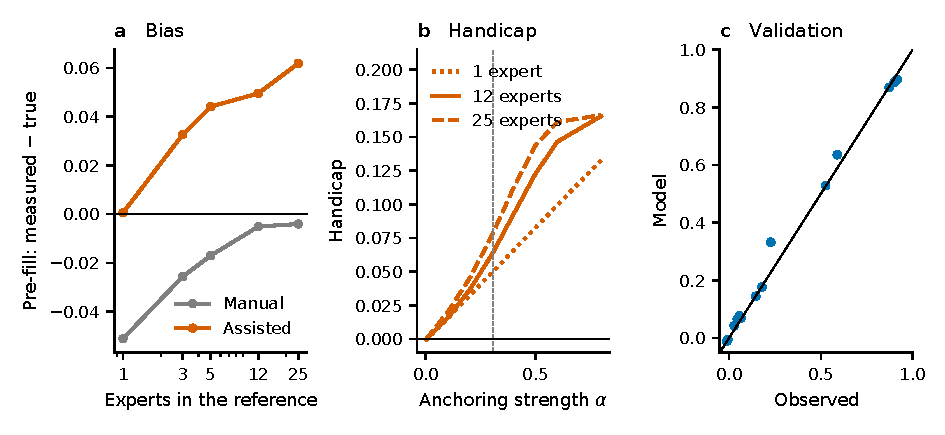
\includegraphics[width=\linewidth]{figures/fig_simulation.pdf}
\caption{Simulation with the truth known (calibrated model; outputs are illustrations under the model's conditions).
(a) The pre-fill's measured minus true accuracy against references of 1 to 25 experts (majority consensus), for
manual and assisted references. (b) The handicap in favor of the pre-fill over an equally accurate competitor, against
anchoring strength, for references of 1, 12 and 25 assisted experts; the dashed line marks the calibrated $\alpha$.
(c) Model against observed values for the validation targets.}
\label{fig:s-simulation}
\end{figure}

\bibliographystyle{unsrtnat}
\bibliography{references}

\end{document}
